\documentclass[11pt,a4paper,spanish]{book}
\usepackage{unir} %\usepackage{estilo_unir}

%para gráficos
\usepackage{standalone}
\usepackage{tikz}
%\usepackage{import}
\usepackage{pgf}
\usepackage{pgfplots}
\pgfplotsset{compat=1.16}
\graphicspath{{img/}{../img/}} % Paths por defecto para las imagenes
\usepackage{smartdiagram}
\usepackage{definitions}

% \usepackage{verbatim}
% to use \begin{comment} for block comments

%tablas más presentables 
\usepackage{booktabs}
\usepackage{graphicx}
\usepackage{rotating}
% Siguientes 3 para imágenes compuestas
\usepackage{float}
% \usepackage[caption = false]{subfig}
%\usepackage[export]{adjustbox}

% para usar \currenttime
\usepackage{datetime}

%\usepackage{amsmath}% ya se define en unir.sty
\DeclareMathOperator*{\argmax}{arg\,max}
\DeclareMathOperator*{\softmax}{\textup{softmax}}


% Fix warning \headheigt is to changeso small
%\setlength{\headheight}{14pt}%

% Permitir modularizar el trabajo
\usepackage{subfiles} % recomiendan cargarlo al final del preámbulo

%---------------------------
%título del trabajo y autor
%---------------------------
\title{Detección de caídas con Dispositivos Vestibles y Redes Neuronales Recurrentes}
\author{Aritz Beraza Garayalde}
\date{\currenttime}
%\director{Sonia Valladares Rodriguez}
\director{Claudia Villalonga Palliser}
\nombreciudad{Paris}

%---------------------------
%margenes
%---------------------------
%\usepackage[margin=1.9cm]{geometry}
%---------------------------
%---------------------------
%---------------------------
%--------------------------
\begin{document}
%---------------- 
% overfull hbox : hide messages
%\hbadness=10000
%\the\tolerance,
%\the\pretolerance,
%\the\hbadness,
%\the\hfuzz,
%\the\emergencystretch,
% Second test
%\pretolerance=150
\tolerance=530
%\hbadness=752
%\hfuzz0pt
%\emergencystretch=0em
% underfull vbox fixes::
%\setlength\parskip{1em plus 2pt}
%\setlength\parskip{\baselineskip}



%\selectlanguage{spanish}
\renewcommand{\listfigurename}{Índice de Ilustraciones}
\renewcommand{\listtablename}{Índice de Tablas}
\renewcommand{\contentsname}{Índice de Contenidos}
\renewcommand{\figurename}{Figura}
\renewcommand{\tablename}{Tabla}

\maketitle
\frontmatter
\tableofcontents
\listoffigures
\listoftables

% Posicion original de mainmatter
\mainmatter

%\chapter{Resumen}
\section*{Resumen}
%\subfile{seccion/10-abstract.es.tex}
\documentclass[../tfm.tex]{subfiles}
\begin{document}
En sociedades cada vez más envejecidas aumenta la necesidad de controlar de forma contínua la salud de las personas mayores, y en concreto identificar las caídas, una de las principales causas de mortalidad en personas mayores. A este respecto existen hoy en día soluciones que sirven únicamente a este propósito, altamente intrusivas, o soluciones basadas en un reloj inteligente y una unidad de procesado independiente que reduce la autonomía. En este trabajo se presenta un sistema de detección de caídas que funciona de forma autónoma en un reloj inteligente o smartwatch ofreciendo un alto grado de precisión en un sistema no intrusivo y autónomo como es un reloj de pulsera.

{\bf Palabras Clave:} Detección de caídas, RNN, LSTM, Detección Anomalías 

\end{document}



%\chapter{Abstract}
\section*{Abstract}
% \subfile{seccion/10-abstract.en.tex}
% !TeX root = ../tfm.tex
%\documentclass[../tfm.tex]{subfiles}
%\begin{document}
\begin{otherlanguage}{english}
The need to continuously monitor elder people's health, and specially detect falls, one of the main death causes of this population, increases in an aging society. With this objective, many solutions exist nowadays, but they are either based in expensive propietary single purpose hardware, usually a wearable sensor and an external computer. These devices are expensive, highly obtrusive and restricted to the an area where the sensor can maintain a link with the main computer. This work will present a fall detection system based purely in a smartwatch, integrating in the same unit the capture, detection and alert components. This solution is presented to the user as an unobtrusive and friendly wristwatch.

{\bf Keywords:} Fall Detection, Human Activity Detection, RNN, GRU, Bourke, Outlier detection
\end{otherlanguage}
%\end{document}


\chapter{Introducción}\label{chap:intro}
\documentclass[../tfm.tex]{subfiles}

\begin{document}

\todohide{Resumen esquemático de cada una de las partes del trabajo. Leer esta sección ha de dar una idea clara de lo que se pretendía y las concluseiones a las que se han llegado y del proceso seguido. Es uno de los capítulos mas importantes
}

\subsection{Motivación}
\info{Problema a tratar, posiles causas, relevancia del problema}

Este trabajo resulta de especial interés en el contexto actual en el que las sociedades de los países desarrollados sufren un rápido envejecimiento de sus poblaciones. Las personas mayores son más propensas a las caídas y estas suponen la principal causa de accidentes y hospitalizaciones de personas mayores de 65 años \todo{dharmita2019. Añadir referencia}. El control contínuo de la salud de poblaciones propensas a estos accidentes permite ofrecer atención de calidad a menor coste. En este contexto es especialmente importante la detección de caidas dentro de este marco de control y atención a estos grupos de población de riesgo.

Existen infinidad de dispositivos para la detección de caídas en el mercado. Desde sistemas de propósito específico como las alarmas de detección de caídas en el baño basadas en una correa atada a la muñeca, a sistemas multipropósito basados en dispositivos de captura y otro de procesado por separado, pasando por complejos métodos de captura y procesado de imágenes. Todos estos sistemas adolecen o bien de restricciones geográficas (funcionan o bien en una habitación o entorno geográfico limitado por el alcance de las cámaras o cobertura del enlace radio con la base de procesado) o bien resultan poco prácticos e incluso obtrusivos para un grupo de usuarios que no está acostumbrado a lidiar con la tecnología.

\subsection{Plantemiento del trabajo}
\todohide{¿cómo se puede resolver el problema qué se propone descripción de objetivos en términos generales?}

Hoy en día tenemos a nuestra disposición cada vez más dispositivos \textit{llevables} (por \textit{wearables} del inglés) con sensores conectados a internet. La evolución de la capacidad de cálculo de los microprocesadores y miniaturización de los sensores ha permitido generalizar y extender y popularizar el uso de dispositivos \textit{llevables} al grueso de la sociedad. Estos avances se aprovechan ya parcialmente en algunas soluciones al problema de la detección de caidas. Se utilizan los datos capturados por el acelerómetro de una pulsera de actividad o reloj inteligente ya sea para realizar un procesado analítico de los parámetros medidos y realizar la detección de una caida (por ejemplo buscar una aceleración fuerte y abrupta) o bien para enviar este flujo de datos a un segundo sistema, para realizar la detección mediante modelos complejos con grandes requisitos computacionales. Ambas soluciones tienen sus pros y contras. La primera tiene a su favor la alta disponibilidad al aunar captura y tratamiento en la misma unidad, pero falla al usar algoritmos poco precisos, al contrario que la segunda opción que se aprovecha de la mayor potencia de un segundo centro de cómputo para mejorar la detección a costa de una mayor complejidad en el sistema que impacta negativamente en su usabilidad y disponibilidad. Hay que tener en cuenta que el público objetivo de esta tecnología es un segmento de población con escasos conocimientos de nuevas tecnologías y poco habituado a su uso diario.

Este trabajo propone una salución basada en aprovechar la mejora en rendimiento de los procesadores de sistemas portables como los usados en relojes inteligentes para realizar tanto captura como tratamiento y detección de caídas en la misma unidad. La diferencia con los sistemas ya existentes, es que el algoritmo usado se base en los últimos avances en tecnologías de predicción temporal con inteligencia artificial, redes recurrentes GRU y un mecanismos de atención o eventos para reducir los requisitos computacionales y obtener  un sistema de detección autónomo en quasi-tiempo real que a la vez sea lo menos obtrusivo para el usuario final, como podría ser el simple hecho de llevar un reloj puesto.

El objetivo es por tanto implementar una solución de detección de caídas con alta precisión, siendo esta al menos comparable a la conseguida en sistemas con cómputo externo, que funcione exclusivamente en un reloj inteligente.


\subsection{Estructura de la memoria}
\todo[disable]{qué hay en cada uno de los subsiguientes capítulos}
\todo{Desarrollar}

El siguiente trabajo se estructura con una revisión del estado del arte y literatura relacionada en el capítulo \ref{chap:stateofart}, seguido de la definición de objetivos y de requisitos previos en los capítulos \ref{chap:objetivos} y \ref{chap:requisitos}. Posteriormente nos adentraremos en el desarrollo e implementación de la solución en el capítulo \ref{chap:descripcion} y en el capítulo \ref{chap:eval} evaluaremos el sistema y sus resultados contra soluciones existentes, antes de exponer las conclusiones (capítulo \ref{chap:conclusiones}) y trabajo futuro. Al final en los apéndices detallaremos otros aspectos como el conjunto de datos usado (Ap.\ref{app:dataset}) y la plataforma usada (Ap.\ref{app:plataforma}).

Entre la literatura previa y de referencia a este trabajo introduciremos los sistemas de detección de actividad humana en \ref{sect:sa_har}, los diferentes modelos usados \ref{sa_modelos_analiticos}, \ref{sa_modelos_ml} antes de introducir los modelos híbridos en \ref{sa_modelos_hybridos}. Intruduciremos también las redes neuronales recurrentes como herramienta de procesado de series temporales \ref{sa_rnn} y la problemática de la optimización de modelos \ref{sa_optimizacion} tanto a nivel computacional como de consumo de recursos y memoria.

Estos conceptos se retoman posteriormente para definir los prerrequisitos: plataforma de desarrollo \ref{req_hardware} como herramientas de software \ref{req_tflite} y conjuntos de datos adecuados para entrenamiento y validación de resultados \ref{req_corpus}. Trataremos la situación actual y soluciones disponibles así como las limitaciones y sus posibles soluciones. Trataremos de nuevo el problema de los diferentes tipos de modelos de detección de caídas \ref{req_modelos} relacionando sus capacidades con las limitaciones tanto de los conjuntos de datos como del soporte físico y computacional usado y su adecuación a la solución propuesta.

En las secciones posteriores detallaremos el algoritmo y modelo usado para la detección de caídas \ref{desc_modelo}, estructura \ref{desc_archi}, implementación \ref{desc_impl} e interfaz\todo{añadir referencia} de la aplicación y las optimizaciones implementadas \ref{desc_optim}, para a la postre evaluar tanto la viabilidad del modelo usado respecto a otras implementaciones \ref{eval_modelo}, como la usabilidad de la aplicación y su adecuación al problema a tratar\todo{añadir referencia}.

Finalmente tras presentar los resultados obtenidos analizaremos posibles mejoras futuras al sistema así como alternativas que no ha dado tiempo a explorar en este trabajo

\end{document}


\chapter{Contexto y Estado del Arte}\label{chap:stateofart}
\documentclass[../tfm.tex]{subfiles}

\begin{document}

Históricamente, los modelos de predicción de caídas están íntimamente ligados al estudio del reconocimiento de actividades humanas (\textit{HAR} del inglés \textit{Human Activity Recognition}): discernir a partir de los datos de los sensores qué acción (\textit{AVC} por \textit{Actividad Vida Cotidiana}, o \textit{ADL} por sus siglas en inglés) estaba realizando el individuo. Según \cite[p.10692]{Ozdemir2014} una caída o golpe no es más que otra actividad y deben considerarse una parte de este problema ya que "son eventos que suceden de forma involuntaria e inesperada durante la realización de las mismas".


\section{Detección de actividad humana y caídas}\label{sect:sa_har}

En \cite[p.2]{Anita2020} se recopilan y definen los principios básicos que debería cumplir un buen sistema de deteción de caídas y que replicamos a continuación:

\begin{itemize}
  \item No ser obtrusivos
  \item No restringir la mobilidad del sujeto
  \item Tener baja latencia
  \item Ser capaz de diferenciar caídas de otras actividades humanas
\end{itemize}

En \cite{Musci2020,Anita2020}, se introducen varias clasificaciones de estos sistemas. En el contexto del presente trabajo, resultan de especial interés la rama de los sistemas \textit{llevables}: "Aquellos en los que los sensores usados para la detección se encuentran embebidos en un dispositivo que debe llevar pueto el sujeto, como por ejemplo en una pulsera" \cite[p.3]{Anita2020}. A su vez podemos dividir estos según el tipo de modelo utilizado para analizar los datos \cite{Anita2020,Lim2014}, en "dos acercamientos principales, los basados en cotas o límites y los basados en aprendizaje automático"\cite[p.1]{Lim2014}

\subsection{Modelos Analíticos: cálculos basados en cotas}\label{sa_modelos_analiticos}

Los primeros acercamientos (\cite{fallindex00, Kangas2008}) al problema de la detección de caídas utilizaron modelos matemáticos basados en el análisis de diferentes parámetros físicos como la aceleración vertical, módulo de la aceleración y postura. Como observa \cite{Bagala2012}, estos métodos puedan conseguir buenos resultados aplicados a pruebas de laboratorio o experimentos controlados, pero no en experimentos de uso real. En parte por un sobreajuste de la calibración de los valores al experimento. En general estos métodos contraponen sensibilidad a especificidad o a la inversa, como puede deducirse de los resultados de \cite{Chen2005,Bourke2006,Kangas2008,Vilarinho2015} y verifica \cite{Anita2020}. A pesar de ello, estos métodos siguen siendo ampliamente utilizados hoy en día por la baja complejidad computacional que requieren, lo que permite ser integrados en pequeños dispositivos poco obtrusivos y con bajas latencias, cumpliendo tres de los cuatro requisitos antes mencionados.


Sobre cálculos basados en cotas, tenemos \cite{fallindex00}, Kangas\cite{Kangas2008} lo compara con el uso ya sea de aceleración vertical o modulo de la aceleración y de nuevo obtiene resultados dispares según el tipo de caída simulada.

La posición de los sensores es también importante, como recalcan \cite{Bagala2012, Vilarinho2015}. Ambos usan smartphones o pulseras de actividad en diferentes posiciones para la captura de la aceleración con resultados muy dispares según el tipo de caída o el tipo de experimento. En el caso de \cite{Vilarinho2015} a pesar de introducir las pulseras como instrumento de captura, delega en un equipo externo (en su caso un teléfono) el análisis y detección de caídas, de manera similar a los experimentos conducidos por \cite{Luque2014} quien añade la posibilidad de realizar el cómputo en un servidor conectado a internet.

\info{REFERENCIA PERDIDA:
Luque2014??
Realmente el monitorizado básico no está tan lejos del resto de métodos e incluso son mejores que algunas implementaciones propietarias comerciales.
Recalca: alta variabilidad de los resultados segúl el tipo de caída (están demasiado optimizados para un tipo concreto, no son de uso general), también hace hincapié en los problemas de usabilidad por parte de usuarios no expertos.}

\todohide{
1- Monitorizado básico (usar módulo del vector aceleración y un threshold X )
2- Fall Index (Yoshida,  T.;  Mizuno,  F.;  Hayasaka,  T.;  Tsubota,  K.;  Wada,  S.;  Yamaguchi,  T.  A  Wearable  Computer System for a Detection and Prevention of Elderly Users from Falling. In Proceedings of  the  12th  International  Conference  on  Biomedical  and  Medical  Engineering  (ICBME),  Singapore, Singapore, 7–10 December 2005.  )
3- PerFallD (Dai, J.; Bai, X.; Yang, Z.; Shen, Z.; Xuan, D. PerFallD: A Pervasive Fall Detection System using Mobile   Phones.   In   Proceedings   of   the   8th   IEEE   International   Conference   on   Pervasive   Computing  and  Communications  Workshops  (PERCOM  Workshops),  Mannheim,  Germany,    29 March–2 April 2010; pp. 292–297) (usa también un giroscopio)
4- iFall (Sposaro,  F.;  Tyson,  G.  IFall:  An  Android  Application  for  Fall  Monitoring  and  Response.    In Proceedings of the Annual International Conference of the IEEE Engineering in Medicine and Biology Society (EMBC 2009), Minneapolis, MN, USA, 2–6 September 2009; pp. 6119–6122. )}




\subsection{Modelos de Aprendizaje Automático}\label{sa_modelos_ml}

La segunda gran familia de modelos utiliza técnicas como \textit{K-Nearest Neighbours}, LSM (\textit{Least Square Method} o \textit{Método de Mínimos Cuadrados}), SVM, Detección Bayesiana, DTW y Redes Neuronales aplicadas a la detección con muy buenos resultados como se extrae de \cite{Ozdemir2014}. En \cite[p.6]{Musci2020} se llega a la conclusión de que el uso de la información de la aceleración únicamente es una fuente de información suficientemente fiable para obtener métricas de detección satisfactorias usando una red neuronal recurrente.

Usando inteligencia artificial, Shi \cite{Shi2020} describe un método basado en acelerómetro triaxial llevado en la cintura para predecir caidas, tratando una caida como una actividad humana más y usando métodos similares a los usados para la predicción de actividad humana (CNN). Casilari en \cite[p.17]{Casilari2020} usa una red de 4 capas convolucionales para el mismo fin, y compara el rendimiento sobre multitud de datasets obteniendo que si bien se puede optimizar el rendimiento para un conjunto en concreto logrando resultados de precisión y especificidad del orden del 100\%, es muy costoso generar un modelo que generalice a todos los datasets. A su vez analiza el impacto de otros parámetros como el tamaño de la ventana temporal \cite[p.16]{Casilari2020}, considerando que a partir de 5 segundos no hay ningún beneficio extra en aumentar el tamaño de la ventana. En \cite[p.59]{Hassan2019} usan una ventana de 1s consiguiendo mejorar los clasificadores existentes. Resultado que coincide con \cite[p.2]{Liu2018} que deslimita la duración de una caída entre los 0,4 y 0,8 segundos, demostrando que una frecuencia de muestreo de 21,3Hz es suficiente cuando se utilizan modelos de aprendizaje automático. Madrano \cite{tfall} usa K-NearestNeighbours y SVM para detectar actividad y varios tipos de caídas, mostrando buenos resultados con SVM que además parece ser capaz de distinguir caídas para las que no ha sido entrenado.

Finalmente, en \cite{Anita2020} tenemos un resumen con los últimos avances y resultados. Introduce otras fuentes de información como es el riesgo biológico, o predisposicion a la caída debido a la edad y otros factores de deterioro de la salud.

Varios estudios \cite{Luque2014,Aziz2017,Aziz2017b} llegan a conclusiones similares respecto a la alta variabilidad de los resutlados según el conjunto de datos de entrenamiento usado, especialmente en los métodos basados en cotas. Sin embargo en \cite[p.9]{Aziz2017b} confirma el resultado de \cite[tfall] sobre la mayor capacidad de generalización de los modelos basados en SVM. A la ver que introduce  encuentra que SVM llega a generalizar incluso con tipos de caídas para las que no había sido entrenado. En la segunda obra analiza en más detalle la detección con SVM usando caídas reales y sugiere usar una combinación de métodos basados en cotas junto con técnicas de aprendizaje automático para obtener mejores estimadores.

\subsection{Modelos basados en eventos o híbridos}\label{sa_modelos_hybridos}

Putra \cite{Putra2017} y Lim \cite{Lim2014} definen modelos híbridos que ofrecen una alternativa a los complejos y computacionalmente costosos modelos de aprendizaje automático y a los simples pero poco precisos modelos analíticos aunando las ventajas de ambos. En sus trabajos usan una etapa de detección basada en las propiedades analíticas de una caída y una posterior etapa de clasificación o decisión basada en modelos más complejos obteniendo "Mejores resultados que con el método de cotas simple (...) y una fuerte reducción del coste computacional respecto al uso del modelo HMM únicamente"\cite[p.5]{Lim2014}.

\section{Predicción de series temporales}

El uso de redes neuronales recurrentes para la predicción de series temporales es ampliamente respondido hoy en dia \todo{citar estudios}. Basaremos la etapa de clasificación en la capacidad de predecir episodios conocidos de este tipo de redes.

\section{GRU vs LSTM para predicción de series}\label{sa_rnn}

Respecto al uso de LSTM para detectar anomalías en series temporales, Wang \cite{Wang2020} usa LSTM para identificar anomalías en la señal de un motor (aunque el usa el error de recostrucción de la descomposición y recomposición wavelet de la señal como entrada a una triple red LSTM, nuestro enfoque es el contrario: usar LSTM a modo de transformada wavelet y luego comparar el error de recomposición).

in\cite{Qin2019} estudia el comportamiento de varias redes recurrentes para la predicción de la saturación de oxígeno en el agua y obtiene que las GRU son las que mejores predicciones (menos error) obtienen (Sobre LSTM e incluso RNN bidireccional). Kofi \cite{Koffi2020} compara LSTM y GRU para predecir mercado de valores con topologías muy variadas (número de celdas, de capas, stateless o no) y encuentra que GRU tiene mejor tasa de aciertos teniendo en cuenta el coste computacional (y muchas veces sin tenerlo) y que no siempre tener dos capas de RNN da mejores resultados.

Alicado al problema de la predicción de la actividad humana, Li\cite{Li2019} usa redes con varias capas LSTM bidireccionales usando los datos obtenidos por un acelerómetro y un radar con un dispositivo de captura en la muñeca mientras consigue resultados comparables a las mejores técnicas de clasificación existentes.

\section{Pruning y técnicas para reducir complejidad de modelos}\label{sa_optimizacion}

A pesar de la creciente capacidad de cálculo de los dispositivos llevables, será necesario optimizar el rendimiento del modelo con el fin de conseguir la mayor capacidad de predicción por Hz del sistema. Para ello dispondremos de dos técnicas: \textit{Pruning} y \textit{Cuantificación}.

\subsection{Pruning}
Un modelo de redes neuronales se puede entender como una matriz de pesos que indican la contribción de cada nodo o neurona al resultado final. Es normal que en esa red haya nodos que aporten más información que otros. Este efecto no es necesariamente negativo, la regularización o normalización L1 busca precisamente este efecto para reducir el sobreajuste de la red a los datos de entrenamiento.

Esta diferencia de aportación nos permite realizar una compresión del modelo. Si aceptamos sufrir unas ciertas pérdidas en la capacidad predictiva del mismo, podemos eliminar los nodos de menor peso reduciendo el tamaño de la red y su consumo de memoria. Esta reducción permite además acelerar el modelo y adaptarlo al uso en sistemas embebidos.\todo{Buscar bibliografía formal para: https://www.machinecurve.com/index.php/2020/09/23/tensorflow-model-optimization-an-introduction-to-pruning/}

\todo{Este artículo cita referencias y es ligeramente más técnico.
https://www.machinecurve.com/index.php/2020/09/29/tensorflow-pruning-schedules-constantsparsity-and-polynomialdecay/}

Una de las técnicas más sencillas para realizar esta eliminación de nodos consiste en definir una aportación mínima objetivo y comparar la magnitud de la aportación individual al resultado final, eliminando aquellos que no alcanzan el nivel $\lambda$ deseado
\[
\hat{w_i} = \left\{ \begin{matrix} w_i & :\mbox{si} |w_i|>\lambda\\
  0 & :\mbox{si} |w_i|\leq\lambda\end{matrix} \right.
\]

Esta compresión se puede hacer sobre un modelo ya entrenado (sendo recomendable realizar un nuevo proceso de entrenamiento para balancear los pesos de los nodos existentes y reducir el error introducido) o realizarlo durante el entrenamiento como si de una regularización más se tratara.

En el caso de TensorFlow, el entorno usado para este proyecto, se permite realizar esta regularización durante el entrenamiento de dos formas:

\begin{itemize}
\item Eliminando nodos de forma lineal, o a tasa constante
\item Eliminando nodos de forma polinomial, o a tasa creciente
\end{itemize}

\subsection{Cuantificación}
\warn{citas necesarias}
Entendemos por cuantificación al proceso de discretizar un grupo de valores. En este caso hace referencia precisamente al descenso en la precisión numérica usada para representar los pesos de nodos y valores de entrada y salida de una red neuronal.

La cuantificación de los valores de entrada y salida a la red consiste en reducir el peso de estos valores. Normalmente se normaliza la entrada y se convierte en valores de tipo entero. Tras el paso por la red, a la salida se aplicac la operación inversa para escalar la salida al rango de valores esperado.

Por su parte la cuantificación de la red neuronal realiza una operación similar con los pesos de los enlaces de las neuronas. Reduce la precisión de las representaciones de estos valores consiguiendo un ahorro en recursos y una mejora en tiempo de cálculo al eliminar el requisito de usar unidades de coma flotante en sistemas embebidos.


\end{document}

 
\chapter{Objetivos}\label{chap:objetivos}
\documentclass[../tfm.tex]{subfiles}

\begin{document}
\info{Puente entre el estudio y la contribución.}
\warn{
Debe contener:
 objetivo general
 objetivo específico
 metodología de trabajo
 }

 \info{
   Los objetivos deben ser \textit{SMART}

     Specificl (objetivo claro)
     Measurable (se pueda medir el éxito o fracaso)
     Attainable (viable su conecución con el tiempo y recursos disponibles)
     Relevant (que tenga un impacto demostrable)
     Time-related (que se pueda realizar en un tiempo determinado)
 }


\section{Objetivo General}
\info{
Un poco la descripción a grandes rasgos de qué se espera explicado al público general.

Ejemplo: Mejorar el servicio de audio gruía de un museo con una guía interactiva por voz valorada positivamente con un 4/5 al menos.
}

Este trabajo presenta una implementación de un sistema de detección de caídas autónomo sobre un dispositivo vestible del tipo smartwatch con una precisión mayor a la disponible en los sistemas vestibles actuales comparable a la de los sitemas basados en aprendizaje automático.

\section{Objetivos Específicos}

Dividiremos el trabajo a realizar en los siguientes pasos o etapas:
\begin{itemize}
  \item Desarrollar un conjunto de datos para el entrenamiento y validación del sistema final.
  \item Estudiar el comportamiento y características de las señales temporales del acelerómetro a partir del conjunto de datos previamente capturado para parametrizar el sistema (tamaño de la ventana de observación y )
  \item Identificar y establecer un índice o métrica derivada de la lectura del acelerómetro que permita su posterior uso para el reconocimiento de caídas.
  \item Desarrollar un modelo de predicción de la evolución temporal del índice elegido usando redes neuronales recurrentes y evaluar su rendimiento.
  \item Implementar un modelo de clasificación de la actividad humana usando el índice basado en la aceleración y el modelo de aprendizaje automático de los puntos anteriores.
  \item Comparar los resultados del modelo implementado frente a los modelos existentes. Analizar y cuantificar la mejoría aportada sobre los métodos analíticos.
  \item Analizar la viabilidad e idoneidad de la solución propuesta y posibles mejoras
\end{itemize}

\todohide{
Conjunto de objetivos más específicos alcanzables por separado. suelen sor los diferentes pasos a seguir para conseguir el objetivo general. Han de ser smart, los verbos deberian ser:     • Analizar
Calcular
Clasificar
Comparar
Conocer
Cuantificar
Desarrollar
Describir
Descubrir
Determinar
Establecer
Explorar
Identificar
Indagar
Medir
Sintetizar
Verificar}

\section{Metodología de trabajo}

\todohide{
Debe describir los pasos que se van a dar, el por qué de cada paso, instrumentos a utuilizar y cómo se van a analizar los resultados.
}

\begin{enumerate}
  \item Generar un nuevo dataset \footnote{Se implementa una app para ello, y se realiza un procesado de los datos obtenidos}
  \begin{enumerate}
    \item Los existentes se basan en detección de actividades
    \item Los pocos basados en detección de caidas se restringen a un subconjunt de caidas muy específico y muchas veces con posiciones del elemento de detección diferente de la usada en el estudio
  \end{enumerate}

  2- Estudiar el dataset obtenido
  a- comprender mejor el comportamiento de las señales capturadas
  b- buscar parámetros importantes para llevar a cabo la detección

  \item Implementar un sistema basado en LSTM y detección de anomalías usando errores de predicción. Mecanismo atencional basado en potencia de señal de entrada?
  \begin{itemize}
    \item Implementar una red LSTM FORWARD, y/o una FORWARD-BACKWARD, Asi como un sistema basado en threshold (usar GRU con RELU para mejorar la eficiencia de cómputo)
    \item Una vez entrenados los modelos con información de actividad ordinaria:
    \begin{itemize}
      \item Implementar una app que o bien en tiempo real o cuando detecte un cierto nivel de actividad lance los modelos de predicción
      \item Usar un sistema que comparando la señal real y la predicha decida si es una "anomalía" o no, lo más básico un RMS del error de predicción.
    \end{itemize}
  \end{itemize}

  \item Comparar los resultados con el estado del arte
  \begin{itemize}
    \item Entrenar el sistema usando al menos un dataset que incluya caídas.
    \item Compararar con al menos métodos de cota fall index y modulo aceleración.
    \item Comparar con estudios previos que usen el mismo dataset.
    \item Analizar los resultados con el dataset propio.
  \end{itemize}

  \item Prueba en uso real. (Si da tiempo)
  \begin{itemize}
    \item Entrenar el sistema con dataset creado.
    \item Usar en interno
    \item Probar en caídas simuladas
    \item Si es posible conseguir ejemplos de caídas reales (app debe enviar todos los eventos registrados como caídas e indicar si han sido confirmados, rechazados o ignorados)
  \end{itemize}


\end{enumerate}


\end{document}


\chapter{Identificación de requisitos}\label{chap:requisitos}
% !TeX root = ../tfm.tex
%! TEX root = ../tfm.tex

\begin{comment}
info{Indicar el trabajo previo realizado para guiar el desarrollo del software.
Debe identificar adecuadamente el problema a tratar, contexto adecuado de uso y funcionamiento de la aplicación. Idealmente se debería realizar con expertos en la materia a tratar.}

todo{referenciar los requisitos de un sistema de detección de caídas, en detalle si es posible}
\end{comment}

En este capítulo presentaremos al lector una serie de desarrollos previos sobres que serán utilizados o sobre los que se asentará el sistema de detección de caídas. Esta selección es fruto de las decisiones tomadas tras una etapa de estudio del estado de la tecnología en el área de detección de actividad humana y análisis de diferentes opciones de materiales, servicios, técnicas, modelos y datos disponibles. Todos los desarrollos aquí presentes fueron seleccionados a priori, antes de iniciar cualquier otra etapa de desarrollo, basándonos únicamente en los requisitos y necesidades del sistema. En los capítulos sucesivos se hará mención y justificación del uso o ausencia en la implementación final de todas estas herramientas.

\section{Plataforma y Entorno de Desarrollo}\label{sec:req:plataforma}

Tras adquirir información de entorno y con el fin de acotar y restringir las opciones disponibles de cara a la elaboración del algoritmo a emplear es necesario determinar sobre qué plataforma o dispositivo va a ejecutarse la aplicación. Esta decisión impondrá nuevas restricciones tales como tipos de fuentes de información/sensores disponibles, frecuencias de muestreo, precisión y magnitud, posición del dispositivo, entorno de programación a utilizar. 

Entre los requisitos que debe cumplir el sistema destacamos principalmente:

\begin{itemize}
  \item Autónomo: Integrar en una única unidad la capacidad de adquisición, cómputo y alerta.
  \item No ser obtrusivo: El dispositivo no debe interferir o limitar la actividad cotidiana del usuario final.
  \item Programable: El dispositivo debe permitir la ejecución de código de terceros, no debe ser una plataforma cerrada.
  \item Capaz de ejecutar modelos de redes neuronales/aprendizaje automático.
\end{itemize}

Se tendrán en cuenta además de cara al cribado final otros criterios como el coste y la preferencia del autor sobre los entornos de programación a usar así como la adaptación al público objetivo: personas mayores de 65 años. Este grupo de población es más reacio al uso de sistemas computerizados por no estar familiarizados con su uso. Así se buscará ofrecer un sistema que reemplace un objeto de uso cotidiano, con una experiencia de usuario equiparable a la de este objeto y que evite cualquier tipo de interacción que no existiera previamente para la manipulación del objeto original. 
  
\subsection{Dispositivo físico}\label{sub:req:hardware}

Analizamos en primera instancia los 

\subsubsection{Tipos de dispositivos analizados}

\paragraph{Teléfono} o \textit{Smartphone}. Un aparato que se ha vuelto ubicuo en nuestra sociedad. Con gran capacidad de cálculo y multitud de sensores. Según la firma \textit{Kantar}(\url{https://www.kantarworldpanel.com/global/smartphone-os-market-share/}) el 99,99\% de los teléfonos vendidos en españa en los 9 primeros meses de 2020 fueron smartphones con IOS o Android y por ende fácilmente programables y con soporte para ejecutar múltiples entornos de modelado de sistemas de aprendizaje automático. Sin embargo adolecen de una complejidad extra: no es un dispositivo que se lleve vestido, y es fácil que el usuario final no lo lleve siempre consigo. Además, en los grupos de poblaciones de edad muy avanzada donde su uso no está generalizado, se convierte en un elemento ajeno y que puede generar rechazo o olvido en su uso.

\paragraph{Chalecos, cinturones y bandas} y otras prendas de vestir han sido usadas con anterioridad \cite{Liu2020, MobiFall} para situar los sensores. La falta de soluciones comerciales disponibles obligaría a desarrollar una plataforma personalizada y por tanto adaptada a los requisitos. Sin embargo este acercamiento se considera altamente intrusivo tanto por limitar al usuario en su vestimenta así como por servir únicamente cuando el usuario lleve puesto el complemento de ropa especificado. Además, la manipulación del mismo no es evidente, pues requiere de una manipulación muy diferente a la prenda de vestir original. 

\paragraph{Pulseras de actividad y Relojes inteligentes}. Hace tiempo que las podómetros evolucionaron gracias a la mejora en la miniaturización de sensores, baterías y microprocesadores en sistemas avanzados de medida no ya de la cantidad de pasos sino de otros muchos parámetros como pulso, oxígeno en sangre, temperatura corporal y orientación. Por su parte, el paso de los relojes computadoras interconectadas y programables se ha realizado más recientemente. Actualmente puede resultar difícil distinguir en la oferta disponible entre un \textit{smartwarch} (reloj inteligente) y una pulsera. Muchas veces es la propia definición del fabricante la que especifica su tipo, por criterios tan dispares como la producción tradicional de la empresa (así pues, Fossil llamará a sus productos relojes inteligentes, mientras otro dispositivo de similares características y formato de la marca FitBit será llamado pulsera por la marca). Al existir tal variedad de oferta es fácil encontrar dispositivos que cumplan con los requisitos de sensores, capacidad de cálculo y de ser programado, así como soporte para entornos de aprendizaje automático. Al tener apariencia de un reloj de pulsera, resultan un soporte ideal: son dispositivos de uso cotidiano, con una manipulación sencilla, y que se llevan siempre puestos. Con el interés de buscar un sistema lo más transparente de cara al usuario posible nos decantamos por esta opción, a pesar de conocer las limitaciones del uso de la muñeca como fuente de información de la aceleración para la detección de actividades \cite{Chen2005} .

\subsubsection{Relojes Inteligentes WatchOS}

A la hora de definir las familias en las que subdividir este tipo de dispositivos encontramos que por norma general cada fabricante ha decidido crear su plataforma única. Tan solo el sistema operativo WearOS parece ser utilizado por varios fabricantes diferentes. No descartamos la opción de implementar una solución propietaria, por lo que también analizamos algunas de los sistemas de microcontroladores más extendidos.

\tablan{tab:familias_smartband}{Familias de Relojes Inteligentes y Pulseras de Actividad}{p{0.20\textwidth}p{0.1\textwidth}p{0.20\textwidth}p{0.35\textwidth}}{
  \emph{Plataforma} & \emph{Progr.} & \emph{Soporte AA} & \emph{Notas} \\ \midrule
  Garmin     & No & No &  \\
  FitBit     & Si & No & \\
  Huawei     & No & No & \\
  TizenOS(Samsung) & Si & \makecell[l]{\tabitem TensorfFlow-lite} & Puede soportar otros entornos como Caffe2, PyTorch pero han de ser portados por el desarrollador \\
  WatchOS(Apple) & Si & \makecell[l]{\tabitem CoreML\tnote{1}} & PyTorch, Tensorflow, Caffe, LibSVM y otros modelos pueden ser importados a CoreML. \\
  Arduino/ESP32 & Si & \makecell[l]{\tabitem TensorFlow-lite} & Muy baja potencia de cálculo y memoria impiden la ejecución de modelos complejos. \\
  WearOS(Google)  & Si & \makecell[l]{\tabitem TensorfFlow-lite\\\tabitem Caffe2\\\tabitem NNAPI\tnote{1}} & Mediante NNAPI permite realizar cómputos intensivos. \\
}{
  \item [1] API para cálculo intensivo que permite portar bibliotecas de Aprendizaje Automático
}{2}

Comparando los requisitos con los resultados de la tabla \ref{tab:familias_smartband} descartamos en primera instancia los dispositivos Garmin, FitBit y Huawei por no permitir el desarrollo de aplicaciones que usen modelos aprendizaje automático. Aunque en teoría sí hay soporte para usar modelos entrenados en las plataformas ESP32/Arduino, al disponer de cantidades de memoria y procesadores poco potentes su uso real queda muy limitado, prácticamente restringido a una mera curiosidad. 

De los tres grupos restantes de dispositivos, la familia de dispositivos WatchOS queda relegada a la tercera posición por su alto precio (hasta 5 veces más caros que los dispositivos de la competencia). La decisión final se decanta finalmente por usar dispositivos WearOS por la preferencia y conocimiento de la plataforma del que ya dispone el autor. 

\subsection{Entorno de Desarrollo}

Nos referimos por entorno de desarrollo al conjunto de herramientas usadas para implementar el sistema. Tanto para el la generación, entrenamiento y análisis de modelos como para la implementación y adaptación del sistema de detección de caídas.



\subsection{Soporte en la Nube}

Si bien el sistema a desarrollar es autocontenido, preveemos la necesidad de implementar una infraestructura de servidor en la nuve para ampliar la funcionalidad y permitir la recopilación de datos, especialmente durante la etapa de recopilación de muestras para crear la base de datos. En concreto buscamos una plataforma de servicios que permita:

\begin{itemize}
  \item Implementar servicios/APIs de forma sencilla.
  \item Sin necesidad de infraestructura para reducir el mantenimiento.
  \item Permita almacenar grandes cantidades de datos.
\end{itemize}

Con estas necesidades en mente seleccionamos la plataforma de servicios en la nube de \textit{Amazon AWS}(\url{https://aws.amazon.com}) dado que además de cumplir con los requisitos mínimos, su amplia popularidad ha permitido crear una comunidad que ofrece un amplio soporte. De toda la oferta de servicios disponibles nos centraremos en el servicio de almacenamiento \textit{S3}, \textit{AWS lambda} para implementar servicios \textit{sin servidor} (sin infraestructura dedicada) y \textit{Amazon API Gateway} para exponer los servicios en Internet. Como extra a valorar cabe destacar la gran cantidad de lenguajes de programación soportados por AWS lambda, lo cual facilitará la implementación al no requerir aprender nuevos lenguajes de programación.

\section{Bases de datos de actividad}\label{sec:req:bases_datos}

Tras la elección tanto de la plataforma física, entorno de desarrollo así como del algoritmo usado, iniciamos la búsqueda de una base de datos que cumpla con los criterios siguientes:

\begin{enumerate}
  \item Contenga datos de la aceleración. Idealmente las 3 componentes espaciales por separado.
  \item Contenga datos tanto de caídas como de otras actividades cotidianas.
  \item La medida de la aceleración se toma desde un sensor en la muñeca.
  \item Contenga resultados de varios sujetos
\end{enumerate}

Tras analizar como se ve en la \autoref{tab:bases_datos} varias bases de datos relacionadas con la detección de actividades cotidianas y caídas. Por la localización de los sensores de medida, la única que cumple los requisitos es UMAFall, sin embargo tiene dos problemas:
\tablan{tab:bases_datos}{Bases de datos de actividad humana}{p{0.2\textwidth}ccccm{0.2\textwidth}m{0.2\textwidth}}{
  \emph{BBDD}    & \emph{Sujetos} & \emph{AHC} & \emph{Caídas} & \emph{Muestras} & \emph{Sensores}      & \emph{Posición} \\ \midrule
  MobiFall\tnote{1}& 24      & 9   & 4      & 630      & \tabitem Acelerómetro \newline\tabitem Giroscopio & Pantalón \\
  MobiAct\tnote{2}& 57      & 9   & 4      & 2526     & Acelerómetro  & Pantalón \\
  tFall\tnote{3}  & 10      & *   & 8      & 10909     & Acelerómetro  & \tabitem Bolsillo\newline\tabitem Bolso \\
  SisFall\tnote{4}& 38      & 19  & 15     & 4505      & \tabitem Acelerómetro\newline\tabitem Giroscopio & Cintura \\
  UMAFall\tnote{5}& 17      & 8   & 3      & 531       & \tabitem Acelerómetro\newline\tabitem Giroscopio\newline\tabitem Magnetómetro & \tabitem Pecho\newline\tabitem Cintura\newline\tabitem Pantalón\newline\tabitem Tobillo\newline\tabitem Muñeca \\
}{
  \item [1]\citeA{MobiFall} 
  \item [2]\citeA{MobiAct} 
  \item [3]\citeA{tfall} 
  \item [4]\citeA{Sucerquia2017} 
  \item [5]\citeA{Edu/UMA/2017} 
  }{2}
\begin{itemize}
  \item Escasez de eventos: tan solo 531 eventos, de 25 categorías reducen el número de instancias por categorías a un promedio de 21. Claramente insuficiente para obtener una cifra significativa.
  \item Poco extendida entre la comunidad. En parte por ser la compilación más reciente, no hemos encontrado estudios suficientes que utilizasen UMAFall para poder realizar una comparación de resultados.
\end{itemize}
Concluimos esta etapa considerando desierta la oferta disponible. Tomamos la decisión de dividir la tarea a realizar en dos ejercicios:
\begin{enumerate}
  \item Implementar, validar, y comparar la viabilidad del algoritmo (independientemente de la plataforma elegida).
  \item Portar el modelo y entrenarlo para la plataforma escogida. 
\end{enumerate}

Esta separación de objetivos permite reducir los requisitos de las bases de datos necesarios para cada uno tal y como recogemos a continuación.


\subsection{Bases de Datos para estudiar el algoritmo}

Al querer únicamente estudiar cómo se comporta el modelo diseñado, no es exigencia la restricción impuesta por el uso de un reloj o pulsera como dispositivo de captura de que los datos sean medidos en la muñeca. Por tanto, estudiando de nuevo la tabla \todo{crear la tabla y poner la referencia} observamos que ahora sí que hay varios candidatos viables.

%SisFALL (Tras considerar otros muchos como umafall, mobiact/mobifall, etc): mayor cantidad de caídas y muchas de las actividades son consideradas \textit{quasi-caidas} y por tanto son casos límite. Si el modelo es capaz de dar buenos resultados en estas condiciones, es un buen modelo. Además, es usado por \cite{Musci2020} y varios de los estudios presentes en \cite{Anita2020} por lo que resulta ideal para comparar los resultados.

\subsection{Base de Datos para la implementación final}

Tras validar el funcionamiento y compararlo con otros modelos en igualdad de condiciones, esta etapa puede realizarse con conjuntos de datos que no dispongan de caídas. Dado que por la naturaleza del modelo propuesto el entrenamiento se realiza únicamente con muestras de actividades cotidianas. A pesar de la existencia de Bases de Datos que cumplen los criterios, se decide finalmente optar por generar un conjunto propio. Al formar parte del desarrollo realizado, trataremos este punto más adelante, en la sección \todo{poner referencia a la sección}. 




\todo{revisar esto}Para poder generar un modelo con el mismo tipo de datos y capturado de la misma forma a los que deberá procesar posteriormente, optamos por realizar un base de datos de datos propio usando el mismo dispositivo sobre el que se ejecutará el prototipo como plataforma de captura.

Este base de datos se realiza usando únicamente información del sensor de aceleración triaxial del reloj Fossil Sport Gen3 \ref{app:fossil} a una frecuencia de muestreo de 50Hz. Los valores de aceleración medidos están expresados en $m/s^2$ dentro de los límites de la plataforma. Este es un base de datos no etiquetado dado que el objetivo es entrenar un modelo de predicción de series temporales y no un clasificador como suele ser habitual.

Para generar las capturas de los acelerómetros se implementa la aplicación \textit{AccelCapture} (\autoref{sec:imp:accelcapture}). En el  \autoref{chap:generar:dataset} se encuentra una descripción del proceso de generación y especificaciones detalladas del base de datos generado.
\todo{no ponerlo como apéndice, es parte importante, ponerlo aquí (referenciar ciertas cosas al apéndice que sean de menor interés)}

A la hora de parametrizar el sistema de captura de datos, optamos por mantener los 50Hz de frecuencia de muestreo. \cite{Liu2018} demuestra que se pueden conseguir buenos modelos basados en aprendizaje automático con tan solo 5,8Hz, aunque generaliza en 21,3Hz la frecuencia de muestreo mínima necesaria. Nos mantenemos por encima de este límite para eliminar una posible fuente de errores en el modelo.





\section{Modelos y Algoritmo}\label{sec:req:modelos}

\todo{nada de vaguedades, qué modelos, cuales voy a usar, qué valores he calculado yo y cuales vienen de fuera}
Estudios similares han mostrado la mayor capacidad de los sistemas basados en aprendizaje automático. Sin embargo estos algoritmos no han conseguido desplazar en los sistemas comerciales a los métodos analíticos por la gran capacidad de cálculo que requieren. Algunos trabajos han demostrado la eficacia de hibridar los modelos usando un modelo computacionalmente simple para realizar una tarea de detección de candidatos a caídas de fondo y un modelo complejo que actúe únicamente sobre este subconjunto de episodios. Este es el acercamiento que toma este trabajo.

\subsection{Modelos Analíticos}

En el apartado \ref{sec:arte:modelos_analiticos} hemos introducido el contexto de este conjunto de algoritmos. Para implementar el sistema necesitamos un modelo simple y de bajo coste computacional y que se base principalmente en los datos captados por un acelerómetro de tres ejes. Dada la situación del sensor, toda medida de la postura queda descartada por no ser aplicable. Finalmente, dado que su función es principalmente la de mecanismo de atención o generador de eventos de posibles caídas es primordial que su sensibilidad sea alta para no perder caídas. La tasa de especificidad modulará la eficiencia del sistema en los planos del tiempo de cálculo y consumo de energía, siendo preferible usar algoritmos con alta especificidad, siempre y cuando no se comprometa la sensibilidad. Tras analizar varios modelos y recopilar los resultados en la tabla \ref{tab:resumen_mod_anal} decidimos optar por la familia de algoritmos propuestos por \cite{Bourke2006} por ser el único que de forma consistente ofrece una sensibilidad del 100\%. Si se observan los resultados de los diferentes algoritmos analizados, se observa la gran varianza de resultados según el estudio que realizase el análisis. Por ejemplo, el algoritmo \textit{Bourke 1} pasa de ser un algoritmo perfecto con una precisión del 100\% a ser inservible por su bajísima especificidad según el conjunto de datos usado. 

\tablan[0.95\linewidth]{tab:resumen_mod_anal}{Características de los modelos analíticos estudiados}{lccccccccll}{
          &       &     & \multicolumn{2}{c}{\emph{Estudio 1\tnote{1}}} &\multicolumn{2}{c}{\emph{Estudio 2\tnote{2}}} & \multicolumn{2}{c}{\emph{Estudio 3\tnote{3}}} & \\
 {\small Modelo}  & {\small Sens.\%} & {\small Esp.\%} & {\small Sens.\%} & {\small Esp.\%} & {\small Sens.\%} & {\small Esp.\%} & {\small Sens.\%} & {\small Esp.\%} & {\small Sensores } & {\small Postura} \\ \midrule
 Kangas 1\tnote{4}  & 100 & -- & 48 & 94 &   &    &   &  & ACC & Si \\
 Kangas 2           & 100 & -- & 48 & 94 & 86 & 98 &   &  & ACC & Si \\
 Kangas 3           & 71  & -- & 31 & 97 & 94 & 94 &   &  & ACC & Si \\
 Bourke 1\tnote{5}  & 100 & 100& 100& 19 & 100& 79 &   &  & ACC & No \\
 Bourke 2\tnote{6}  & 97  & 99 & 72 & 87 & 70 & 99 &   &  & ACC & Si \\
 Bourke 3\tnote{7}  & 100 & 100& 87 & 97 &    &    &   &  & ACC + GYRO & Si \\
 Chen \tnote{8}     &     &    & 76 & 94 &    &    &   &  & ACC & No \\ % ACC & Si
 FallIndex\tnote{9} &     &    &    &    &    &    & 42&95& ACC & No \\
}{
  \item [1] \citeA{Bagala2012}
  \item [2] \citeA{Aziz2017}
  \item [3] \citeA{Vilarinho2015}
  \item [4] \citeA{Kangas2008}
  \item [5] \citeA{Bourke2006}
  \item [6] \citeA{Bourke2008}
  \item [7] \citeA{Bourke2010}
  \item [8] \citeA{Chen2005}
  \item [9] \citeA{fallindex00}
  }{3}



\paragraph{Algoritmo Bourke 1} El modelo de Bourke 1\cite{Bourke2006} se basa en el estudio de la evolución del módulo de la aceleración. Partimos del principio de que todo cuerpo sufre una aceleración constante de $9,8m/s$ o 1G correspondiente a la gravedad terrestre. Como podemos apreciar en la figura \ref{fig:bourke_thresholds}, al principio de una caída, típicamente se produce un descenso en el módulo de la aceleración ya que al caer, la componente vertical contrarresta el efecto de la gravedad. Al impactar posteriormente contra el suelo se produce un pico en la aceleración. El algoritmo de Bourke utiliza esta característica forma para establecer dos niveles para determinar la detección de caídas. Estas cotas se denominan \textit{LFT} (Nivel de caída inferior) para el nivel mínimo de aceleración medido y \textit{UFT} (Nivel de caída superior) para el nivel superior. El algoritmo de Bourke considera que se ha producido una caída cuando en un intervalo determinado de tiempo se rebasan ambos límites. 

El proceso para elegir estos límites garantiza que por construcción la sensibilidad del algoritmo sea del 100\% sobre la base de datos elegida. Para ambos límites, se recorre todo el conjunto de datos y se busca entre todas las caídas:
\begin{itemize}
  \item El mayor de los mínimos de aceleración de las caídas (para definir \textbf{LFT})
  \item El menor de los máximos de aceleración de las caídas (para definir \textbf{UFT})
\end{itemize}

Garantizando así que todas las caidas del conjunto de datos serán detectadas, y por tanto la sensibilidad siempre sea máxima. Por contra esto hace que el valor de especificidad del algoritmo sea altamente dependiente del resto de actividades incluidas en la base de datos. Esta característica explicaría la gran disparidad de resultados de la tabla \ref{tab:resumen_mod_anal}. 

\figura{BourkeThresholds}{fig:bourke_thresholds}{Detalle del modelo de detección de Bourke}

Recogemos en la tabla \ref{tab:bourke_threshold_values} una lista con los diferentes valores obtenidos para LFT y UFT según diversos estudios. Su valor es claramente orientativo dada la dependencia de la base de datos usada, que nos obligará a obtener estos valores nuevamente durante la implementación para adaptarlos a SisFall.

\tabla[0.43\linewidth]{tab:bourke_threshold_values}{Valores UFT y LFT de Bourke por estudio}{llcc}{
  \emph{Estudio} & \emph{Posición} & \emph{UFT} & \emph{LFT} \\ \midrule
  \citeA{Bourke2006} & Pecho & 3,52g & 0,41g \\
                     & Cintura & 2,74g & 0,60g \\
  \citeA{Bourke2010} & Cintura & 2,80g & 0,65g \\                   
  \citeA{Bagala2012} & -- & 1,79g & 0.73g \\
}{2}


\subsection{Modelos Basados en Aprendizaje Automático}

\subsection{Modelos Híbridos}

\section{Biblioteca de Modelos Neuronales} \label{sec:req:tflite}

Una de las piezas angulares de todo el desarrollo es la generación y entrenamiento del modelo. Si bien es factible realizar una imlementación directa tanto del modelo como de las funciones de entrenamiento, no es óptimo ni recursos ni en resultados. Existen multitud de de bibliotecas para el desarrollo, entrenamiento y despliegue de modelos de los que citamos brevemente los más extendidos:

\paragraph{Caffe2 y PyTorch}

Caffe2 (\url{https://caffe2.ai/}) Es en su origen una biblioteca de modelos neuronales centrada en la velocidad con soporte para el lenguaje de programación \textit{python}. Desde hace 2018 forma parte de la biblioteca PyTorch (\url{https://pytorch.org/}). PyTorch auna un módulo de cálculo de tensores y uno de modelado de redes neuronales con gran énfasis en la aceleración mediante GPU. Es, junto con TensorFlow, la biblioteca de Modelos Neuronales más usada en el ámbito académico.

\paragraph{TensorFlow + Keras}

Similar al caso anterior, Keras (\url{https://keras.io/}) es un módulo que ofrece una API de alto nivel para facilitar la generación y entrenamiento de modelos. No es en si una biblioteca de redes neuronales sino una interfaz de alto nivel a varias de estas como TensorFlow, Theano, CNTK y otros. TensorFlow es al igual que PyTorch una biblioteca de cálculo de tensores y de modelado de redes si bien sus algoritmos están optimizados para ejecutarse sobre unidades TPU también soportan aceleración en GPUs. Desde la versión 2.0 de TensorFlow, se incluye Keras para ofrecer tanto una API de bajo nivel como otra de alto para la generación de modelos. Al ser propiedad de Google, la integración con sus productos es de las mejores. Dispone de un módulo para la ejecución de modelos en plataformas embebidas.

\paragraph{SciKit-Learn}

Scikit-learn (\url{https://scikit-learn.org/}) se presenta como una biblioteca de funciones de tratamiento de datos. Ofrece imlementaciones de funciones y algoritmos de aprendizaje automático muy variados como \textit{random forest}, \textit{SVM}, textit{K-NN} y otros, así como funciones para el pre-procesado de datos. Soporta también modelos de redes neuronales, aunque su API de desarrollo des de muy alto nivel y dificilmente industrializable.

La elección del sistema WearOS para imlementar la aplicación, unida a la popularidad tanto en el ámbito académico como profesional así como el soporte y optimización para sistemas embebidos hace que nos decantemos por la opción TensorFlow + Keras.

\section{Optimización de modelos}\label{sec:req:optimizacion}

Los modelos basados en redes neuronales adolecen generalmente por su gran tamaño y la necesidad realizar infinidad de cálculos. Estos problemas se acrecentan cuando el objetivo es usar el modelo en un sistema embebido con poca memoria y microprocesadores optimizados para el consumo de energía en lugar de potencia de cálculo. Esta escasez de recursos obliga a la \textit{optimización} del algoritmo y modelo usados. Entendiendo por optimización la reducción de complejidad controlada para conseguir un modelo que requiera menor capacidad de cálculo y memoria. Estas técnicas tendrán todas un impacto en la precisión del sistema por lo que el objetivo es conseguir un equilibrio entre la degradación de la capacidad predictiva y la reducción de la latencia debida al menor coste computacional. Establecemos dos criterios previos a cumplir por el sistema final:

\begin{itemize}
  \item Arbitrariamente escogemos una latencia máxima de 1 segundo desde el instante del primer impacto.
  \item La elección de la plataforma nos limita tanto en velocidad de cálculo como en tamaño al disponer únicamente de 512MBytes de memoria RAM.
\end{itemize}

\subsection{Técnicas de Optimización: Pruning y Cuantificación}

  A pesar de la creciente capacidad de cálculo de los dispositivos vestibles, será necesario optimizar el rendimiento del modelo con el fin de conseguir la mayor capacidad de predicción por Hz del sistema. Para ello dispondremos de dos técnicas: \textit{Pruning} y \textit{Cuantificación}.

\subsubsection{Pruning}

Si añadimos que indican la contribción de cada nodo o neurona al resultado final. Es normal que en esa red haya nodos que aporten más información que otros. Este efecto no es necesariamente negativo, la regularización o normalización L1 busca precisamente este efecto para reducir el sobreajuste de la red a los datos de entrenamiento.


Si pensamos en reducir el tamaño de una red neuronal, probablemente una de las soluciones que nos venga a la cabeza sea sea hacer un \textit{tree-shacking}, eliminar aquello que no se necesita. El término, usado en ciencias de la computación se aplica para reducir el tamaño de aplicaciones al eliminar el código que no es utilizado. Podemos pensar en realizar un cribado similar en la red eliminando aquellos pesos menos relevantes para la salida. Propuesto en \citeA{Mozer1989} como una herramienta para simplificar las redes de neuronas y facilitar así la comprensión de su funcionamiento, acelerar el aprendizaje al reducir el tamaño de la red y por la misma razón facilitar la capacidad de la red de generalizar. La técnica propuesta consiste en medir la influencia de los nodos en la señal de salida: comparar el resultado con y sin el nodo activado. Sabiendo la influencia de la aportación de cada nodo podemos determinar un umbral y eliminar los nodos con menor contribución reduciendo la red. \citeA{Yann1989} confirma que además de conseguir reducir el tamaño de la red a la mitad, el aprendizaje de la misma puede llegar a mejorar.


Recordemos, una capa de una red neuronal se puede modelar mediante la ecuación $H_i = f_i(W_ix+B_i)$ donde tenemos una matriz de conexiones $W_{i}$ y una matriz de sesgos $B_{i}$ y la función de activación $f_i(x)$. Si añadimos varias capas sucesivas podemos deducir que el impacto de un nodo, especialmente en las primeras capas de la red crecerá con cada capa posterior. Sin embargo eso no es así ya que en muchos casos la aportación puede quedar neutralizada por sucesivas inversiones de signo en el resto de capas, o resultar que el nodo se activa prácticamente con el mismo valor o que las capas posteriores estén en el límite de la función de activación y su influencia sea prácticamente irrelevante\cite{Mozer1989}. Es más, posiblemente el lector haya rápidamente asociado por su similitud esta técnica con una regularización mediante \textit{dropout}. Las similitudes son evidentes, pero hay sin embargo diferencias importantes:
\begin{itemize}
  \item Los nodos anulados o eliminados se pierden de forma definitiva
  \item Los nodos se seleccionan de acuerdo a su aportación y no de forma aleatoria
\end{itemize}

A la hora de aplicar una técnica de pruning sobre la red es necesario entender que tras cada etapa de eliminación de nodos debe realizarse una etapa de reajuste de la red resultante para corregir el efecto de la pérdida de las neuronas. Este reajuste o aplanamiento de la red resulta especialmente efectivo en redes con múltiples capas como demuestra \citeA{Cai2020} logrando reducir el tamaño de \textit{ResNet110} en un 30\% y un descenso de la precisión de la red del 0,15\% y la reducción del número de operaciones necesarias a la mitad. Otros estudios\cite{Lee2019,Bartoldson2019,Han2015} confirman estos resultados y presentan una novedad: Las grandes reducidas mediante pruning presentan mejores resultados que los modelos pequeños (ResNet32 tras ser comprimida es mejor clasificando imágenes que WRN16, a igual número de nodos). Básicamente, se mantiene la mayor capacidad de generalización o aprendizaje del uso de mayor número de capas incluso al reducir el número de neuronas.

Esta técnica, junto con la cuantificación de los valores, se presenta como una herramienta imprescindible para lograr los objetivos de nuestro sistema. Tensorflow permite aplicar prunning a los modelos, aunque el único algoritmo disponible, \textit{prune low magnitude} sea similar al básico definido por \citeA{Mozer1989}: eliminar aquellos nodos cuyo peso sea menor que un determinado nivel.
\[
  pruned(w_{i})=\left\{
    \begin{array}{lcl}
      w_i & si & |w_i| > \lambda \\
      0 & si & |w_i|\leq  \lambda
    \end{array}
    \right.
\]

Este proceso se va realizando durante un número determinado de iteraciones de entrenamiento durante el cual se van anulando progresivamente una cantidad determinada (ya sea un número fijo o una evolución polinomial) de nodos en cada etapa de entrenamiento. \cite{Yann1989} Los modelos son cada vez más comlejos y con el aumento en complejidad de problemas seguirán crecienco. Un método que elimina nodos permite no solo mejorar la capacidad de generalizar 

\begin{comment}

  https://www.machinecurve.com/index.php/2020/09/23/tensorflow-model-optimization-an-introduction-to-pruning/
  ligeramente más técnico.
https://www.machinecurve.com/index.php/2020/09/29/tensorflow-pruning-schedules-constantsparsity-and-polynomialdecay/
\end{comment}


\subsubsection{Cuantificación}

Además de eliminando nodos de la red, hay otra técnica que permite reducir el tamaño y requisitos de esta: reducir el número de bits usados para representar las conexiones y sesgos. Entendemos por cuantificación al proceso de discretizar un grupo de valores. En este caso en concreto hace referencia al mencionado descenso en la precisión numérica usada para representar los pesos de nodos y valores de entrada y salida de una red neuronal.

Una de las primeras aproximaciones a la cuantificación de los parámetros de redes neuronales aparece en \citeA{Courbariaux2015}. \citeauthor{Courbariaux2015} busca una solución al problema de los crecientes requisitos de potencia de cálculo necesarios por los modelos de redes de neuronas. Esta optimización espera reducir la dependencia en la mejora de las unidades GPU(\textit{Graphics Processing Unit}) y CPU, hasta ahora uno de los principales factores que limitan evolución en este área. \cita[{\citeNP[p.~1]{Courbariaux2015}}]{La mayoría de los cálculos realizados en el entrenamiento y aplicación de una red neuronal consisten en multiplicar un peso determinado por valor real por una activación definida por un valor real}, así pues decide binarizar tanto pesos como activaciones y reducirlos a solo dos valores: $0$ y $1$ o $+1$ y $-1$. Los resultados obtenidos son esperanzadores, una reducciónd el tamaño a 1/16 del original (de 16 bits usados para representar pesos y activaciones pasa a uno único) y una mejora en la velocidad de respuesta de la red tres veces menor.

La reducción en el tamaño de la red es evidente. Si tenemos $N$ parámetros en una red representados con $m$ bits cada uno, el tamaño final de la red es $S(red)=Nm$ es por tanto una dependencia lineal. La mejora en los tiempos de cómputo es más complejo. Trabajar con números reales, o de coma flotante, requiere de unidades de cálculo especializadas, ya sean GPUs o unidades de coma flotante en CPUs. Este requisito de unidades especializadas es determinante en el rendimiento, pues será determinante en la velocidad de cálculo del modelo. Esta problemática la estudia en detalle \citeA{Vanhoucke2011} buscando optimizar la velocidad de los modelos. Se fija en la lentitud de las unidades CPU para realizar grandes cantidades de cálculos en coma flotante y propone en este caso usar valores enteros. Predice que el impacto negativo será mínimos pues \cita[{\citeNP[p.~5]{Vanhoucke2011}}]{las activaciones son probabilidades, limitadas al rango $[0:1]$ así pues no hay riesgos relacionados con el escalado al usar enteros. Y como la entrada de cada nodo es la salida de una activación esto asegura que el rango de valores permanecerá acotado}. Aplicando cuantización para convertir los pesos de reales a enteros, y otras optimizaciones en la implementación, consigue reducir a menos de un tercio el tiempo de respuesta de una red de procesado del habla con un error de precisión añadido inferior al 0,1\%.

Hasta ahora hemos tratado pesos y activaciones como un todo: aplicamos la misma regularización o reducción de precisión a ambos conjuntos de valores por igual. A esta técnica se la conoce como \textit{Cuantificación de precisión uniforme}, en contraste con la \textit{Cuantificación de precisión mixta}. Este última propone tratar la reducción de tamaño de cada conjunto de valores por separado, consiguiendo una mayor reducción del tamaño con un impacto menor en la precisión del modelo \cite{Jin2019} e incluso a veces mejorando el rendimiento. 

El resultado del último párrafo, de nuevo, no habrá pillado desprevenido al lector que rápidamente asocia la reducción en la precisión con un aumento del ruido, al que llamamos \textit{ruido de cuantificación} y por tanto similar a una regularización de la red por ruido \cite{Bishop1995,Noh2017}. Esta capacidad de regularización de la red resultante de la cuantificación y entrenamiento de los pesos de la red es utilizado directamente por \citeA{Wu2019} no ya con el objetivo de mejorar el tamaño y velocidad del modelo sino para mejorar su capacidad de aprendizaje y generalización mejorando la capacidad de clasificación de imágenes de una red en hasta un 10\%. 

TensorFlow Lite ofrece diversas opciones para realizar la cuantificación de modelos como presenta la tabla \ref{tab:tflite_quantization}. En resumidas cuentas ofrece dos opciones: realizar la cuantificación sobre modelos ya entrenados o realizarlo durante el entrenamiento del modelo. Este segundo tipo ofrece mejor granularidad y fiabilidad ya que permite definir secciones específicas del modelo que no sean alteradas y asegura que los rangos y escalados de se realizan teniendo el cuenta todos los datos disponibles. 


\tablan{tab:tflite_quantization}{Detalle de los tipos de cuantificación disponibles en TensorFlow Lite}{llcccl}{
  Técnica                   & Datos Requeridos  & Compresión  & Precisión & Velocidad & Hardware Soportado \\ \hline 
  Float16\tnote{1}          & -                 & \~50\%      & 0         & --        & CPU, GPU \\
  Rango Dinámico\tnote{1}   & -                 & \~75\%      & ---       & x2,5      & CPU, GPU \\
  Enteros\tnote{1}          & Si\tnote{3}       & \~75\%      & --        & x3        & CPU, GPU, TPU, DSP \\
  QAT\tnote{2}              & Si\tnote{4}       & \~75\%      & -         & x3        & CPU, GPU, TPU, DSP \\
}{
  \item [1] Cuantificación post-entrenamiento.
  \item [2] \textit{Quantification Aware Training} (Entrenamiento Para Cuantificación), cuantificación se prepara durante el entrenamiento. 
  \item [3] Es necesario proveer un subconjunto representativo de datos.
  \item [4] Se usa todo el conjunto de entrenamiento.
  }{3}

La precisión y número de bits usado para representar los pesos y activaciones puede verse en la tabla \ref{tab:tflite_weights_activations}. La cuantificación a enteros y OAT resultan en redes con el mismo peso, la diferencia entre ambos es cómo se calculan y escalan los valores (Enteros usa un subconjunto de datos, lo cual penaliza su precisión, contra el uso de toda la base de datos de entrenamiento como hace OAT), y en que OAT al realizarse durante el entrenamiento permite compensar el error introducido, funcionando, como ya hemos mencionado, como una regularización.

\tablan[0.55\linewidth]{tab:tflite_weights_activations}{Tipos de representación usados en cada técnica}{lcc}{
  Técnica & Pesos & Activaciones \\ \hline
  Float16 & Float(16bit) & Float(16bit) \\
  Rango Dinámico & Entero(8bit) & Entero(8bit)\tnote{1} \\
  Enteros & Entero(8bit) & Entero(8bit) \\
  Enteros Experimental & Entero(8bit) & Entero(16bit) \\
  OAT     & Entero(8bit) & Entero(8bit) \\
}{
  \item [1] Las activaciones se convierten de coma flotante a entero al vuelo y el resultado se almacena en coma flotante
  }{2}

  La combinación de estas técnicas, no solo es posible, sino deseable para conseguir reducir el consumo de recursos, memoria, consumo energético y tiempo de proceso, en órdenes de magnitud. El uso de Pruning y Cuantificación permite reducir grandes redes a una fracción: VGG16 se comprime de los 552MBytes originales a apenas 11,3MBytes, Alex-Net adelgaza de 240MBytes hasta los 6,9MBytes ambas sin pérdida de precisión\cite{Han2015}. Respecto a los tiempos, según \citeauthor{Han2015}, en un chip integrado para móviles los tiempos de ejecución son en promedio 4,2 veces más rápidos. Dados estos resultados previos, esperamos que estas técnicas tengan un gran impacto a la hora de permitir la ejecución de modelos de calidad de manera eficiente.














La cuantificación de los valores de entrada y salida a la red consiste en reducir el peso de estos valores. Normalmente se normaliza la entrada y se convierte en valores de tipo entero. Tras el paso por la red, a la salida se aplicac la operación inversa para escalar la salida al rango de valores esperado.

Por su parte la cuantificación de la red neuronal realiza una operación similar con los pesos de los enlaces de las neuronas. Reduce la precisión de las representaciones de estos valores consiguiendo un ahorro en recursos y una mejora en tiempo de cálculo al eliminar el requisito de usar unidades de coma flotante en sistemas embebidos.




% \end{document}



\chapter{Generación de la base de datos}\label{chap:generar:dataset}
% !TeX root = ../tfm.tex
%! TEX root = ../tfm.tex

En este capítulo expondremos las tareas realizadas para obtener una base de datos propia para el posterior entrenamiento del sistema, así como la descripción de la misma y de los estudios previos de las tramas obtenidas que nos ayudarán en el capítulo siguiente a la definición del modelo y parámetros del algoritmo.

Como ya hemos presentado anteriormente en la sección \ref{sec:req:bases_datos}, nos encontramos ante la falta de una base de datos para entrenar el modelo del producto final. Al tratarse de un modelo experimental es necesario conseguir un conjunto de datos lo más parecido posible a los capturados por la plataforma física utilizada. A su vez es necesario validar la capacidad de esta plataforma para servir al propósito de este trabajo. Así, con esta doble tarea de generar una bases de datos y confirmar que la plataforma cubre nuestras necesidades funcionales realizamos el primer desarrollo propio del trabajo.

\section{Captura de datos: AccelCapture}\label{sub:imp:accelcapture}

\textit{AccelCapture} es el nombre del sistema de captura de tramas de la aceleración capturada por el sensor situado en un reloj inteligente con sistema operativo \textit{WearOS}. Consta de dos componentes: una unidad de adquisición de datos, el propio reloj, y una segunda unidad de almacenamiento situada en la nube. Tal y como puede apreciarse en el diagrama de clases de la figura \ref{fig:accelcaptureClasesUml} la aplicación en si misma se compone de tres bloques funcionales.

\figura[0.47]{accelcaptureClassUML}{fig:accelcaptureClasesUml}{Diagrama de clases de AccelCapture}

\paragraph{MainWearActivity}
El punto de entrada de la aplicación. Genera la interfaz de usuario y permite introducir el nombre el usuario a la vez que verificar el estado del servicio de captura de datos e iniciar o parar su ejecución.

\paragraph{SensorsReader}
Un servicio que al ser creado se registra para recibir eventos y lecturas del sensor de aceleración triaxial del reloj. Posee una cola circular donde almacena los últimos 5 segundos de muestras (si por ejemplo la velocidad de lectura del sensor es de $1/50$, el buffer posserá $50 * 5 = 250$ muestras).
Este servicio realiza el análisis de la aceleración para detectar movimiento según el algoritmo definido en la figura \ref{fig:capturaFlow}. Tras cada muestra el algoritmo evalúa la variación de la aceleración según la fórmula: 

\[
  \Delta A_{i}=\left\{
    \begin{array}{lcl}
      |A_i - g| & si & i = 0 \\
      |A_i - A_{i-1}| & si & i > 0 \\
    \end{array}
    \right.
\]

Donde $g$ corresponde a la aceleración de la gravedad terrestre o $9,8m/s^2$. Este valor $\Delta A_i$ se utiliza para realizar la detección de actividad mediante dos mecanismos:

\figura[0.55]{capturaFlujo}{fig:capturaFlow}{Flujo de trabajo de la aplicación AccelCapture}

\begin{enumerate}
  \item \textbf{Movimiento repentino} Se activa si la muestra leida es mayor de $2g$.
  \item \textbf{Movimiento prolongado} Activado cuando la aceleración promedio del contenido del buffer es superior a $0,3m/s^2$
\end{enumerate}

La cota de detección de movimiento repentino se calcula a partir de los resultados obtenidos por \citeA{Bourke2006} para la medición de la cintura por ser la que menor aceleración registra. La diferencia entre la aceleración de pico y de valle usada por bourke es de $\Delta A = (2,74 - 0,60)g = 2,14g$ redondeando a la baja a $2g$ para garantizar la detección de todos los eventos de este tipo. Finalmente, la cota del detector de actividad prolongada, fijada en $0,3m/s^2$, se mide de forma experimental resultado de promediar el vector para realizar el movimiento de leer la hora en el reloj (figura\ref{fig:accelMirarReloj}) y volver a la posición de reposo durante la ventana de 5 segundos que usa la aplicación. En caso de activarse alguno de estos mecanismos, el servicio considera que ha detectado una actividad y manda el contenido del buffer al servidor para ser guardado. 

\figura{MirarRelojAccel}{fig:accelMirarReloj}{$|A|$ y $\Delta A$ de resultantes de mirar el reloj}

El código de las funciones lambda puede consultarse el el apéndice \ref{app:code:accelcapturelambda} mientras que el de la aplicación AccelCapture está disponible para descarga en \url{https://github.com/aberaza/accelCapture}.

\subsection{Interfaz de Usuario}

La interfaz de usuario de la aplicación permite gestionar y observar el estado del servicio de captura así como definir el identificador de usuario al que pertenece la sesión. Como puede observarse en las capturas de pantalla de la figura\ref{fig:accelcapture:UI} se muestra en la parte inferior de la pantalla un boton con información del estado actual del servicio. El botón al ser pulsado alterna entre los estados \textit{activado} y \textit{desactivado}. En la parte superior de la pantalla se muestra la información del identificador de usuario o \textit{nombre} al que se asociarán todas las sesiones registradas. Este identificador puede modificarse desde el mismo reloj. Una vez activado el servicio de captura, puede esconderse interfaz y volver al modo reloj ya que el servicio sigue trabajando de fondo. 
\begin{figure}[htb!]
  \centering
  \begin{subfigure}[b]{0.4\textwidth}
      \centering
      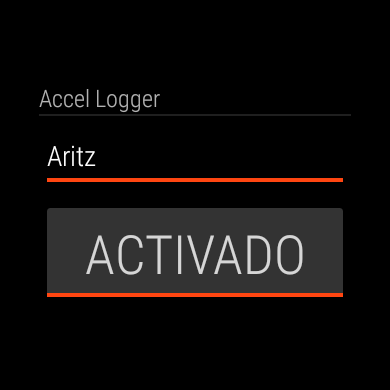
\includegraphics[width=\textwidth]{accelCaptureAct.png}
      \caption{AccelCapture Activado}
      \label{fig:accelCapture:UI1}
  \end{subfigure}
  \hfill
  \begin{subfigure}[b]{0.4\textwidth}
      \centering
      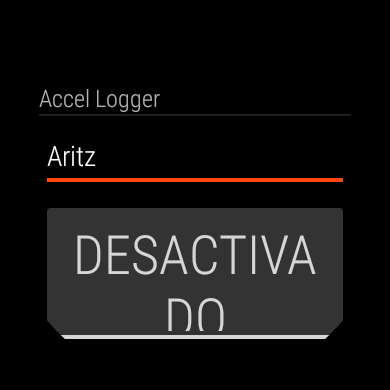
\includegraphics[width=\linewidth]{accelCaptureDes.png}
      \caption{AccelCapture Desactivado}
      \label{fig:accelCapture:UI2}
  \end{subfigure}
  \caption{\label{fig:accelcapture:UI} Interfaz de usuario de AccelCapture}
\end{figure}

\subsection{Almacenamiento de datos}

\tabla[0.65\linewidth]{tab:accelcapture:api}{API del servidor AccelCapture}{llll}{
  Método  & URL         & Carga         & Función lambda    \\ \hline
  POST    & /saveAccel  & AccelSession  & doGuardarAccel()  \\
}\todo{poner la vuena ruta}

Tal y como se menciona en el apartado \ref{sec:req:nube} la plataforma en la nube se implementa usando los servicios de AWS. Para esta función crea un microservicio o \textit{API}(lista de funciones de acceso público que ofrece una biblioteca de programación) ( del tipo \textit{REST}(Arquitectura que implementa una interfaz sobre el protocolo \textit{HTTP}). Este servicio, definido en la tabla \ref{tab:accelcapture:api} se encargará de recibir la llamadas de la aplicación y guardar el contenido en un archivo \textit{JSON} (lenguaje de definición de estructuras de datos que usa la notación de JavaScript).

\subsubsection{Formato de los datos}

La estructura almacenada se muestra en la tabla \ref{tab:accelcapture:accel_session} la denominamos \textit{AccelSession}. Este objeto contiene información sobre el sensor (error y frequencia de muestreo), fecha de la captura así como unos identificadores del usuario y de la sesión además de la información capturada en los tres ejes del acelerómetro.



\begin{table}[h]
  \subtabla[0.48]{tab:accelcapture:accel_session}{Descripción del Objeto AccelSession}{lll}{
Campo           & Tipo Dato     & Descripción \\ \hline
\textit{uid}    & Alfanumérico  & Identificador único de usuario \\
\textit{sid}    & Alfanumérico  & Identificador único de sesión \\
\textit{sensorResolution} & Real & Resolución del sensor (en $m/s^2$) \\
\textit{sensorMaxRange} & Real  & Valor máximo de la medida (en $m/s^2$) \\
\textit{startTime} & Entero     & Tiempo EPOCH del inicio de la sesión (en segundos) \\
\textit{samples}  & Entero      & Número de muestras de la sesión \\
\textit{triggerMethod} & Texto  & Nombre del evento que inició la sesión de captura \\
\textit{sessionData} & SessionData & Estructura con los datos capturados del sensor \\
}{}

%\hspace{\fill}
\subtabla[0.48]{tab:accelcapture:session_data}{Descripción del Objeto SessionData}{lll}{
Campo           & Tipo Dato     & Descripción \\ \hline
\textit{duration} & Entero      & Duración, en $\mu s$, de la sesión \\
\textit{activity} & Texto       & Nombre de la actividad realizada durante la captura \\
\textit{rate}   & Entero        & Ratio de muestreo (en $Hz$) \\
\textit{accelerationX} & Lista<Reales> & Lista de valores de la aceleración capturados en el eje X (en $m/s^2$) \\
\textit{accelerationY} & Lista<Reales> & Lista de valores de la aceleración capturados en el eje Y (en $m/s^2$) \\
\textit{accelerationZ} & Lista<Reales> & Lista de valores de la aceleración capturados en el eje Z (en $m/s^2$) \\
}{right}

\caption{\label{tab:accelcapture:data_types} Estructuras de datos de AccelCapture}
\end{table}


\section{Generación de la base de datos}

Durante un periodo de 6 meses se han realizado capturas de movimiento usando la aplicación AccelCapture en diversos sujetos. Las capturas se realizan llevando el sensor activado 24 horas al día, incluidos los periodos de reposo y sueño, eliminando, de ser necesario, aquellas capturas en las que hubo alguna caida. El objetivo es capturar la mayor cantidad posible de sesiones de actividades diarias ordinarias, así como otros eventos que, a pesar de que el usuario se encuentre estacionario y en reposo, generan una señal de aceleración no constante como puede ser el uso de diferentes modos de transporte (tren, avión, coche, moto). En total se han registrado más de 10 horas de actividad repartidas en 300 sesiones diferentes.

\subsection{Procesado de las tramas}

A la hora de construir la base de datos, se mantiene prácticamente la estructura de información usada para el almacenamiento en el servidor. Los archivos correspondientes a las sesiones registradas se leen y almacenan en un dataframe. No se realiza ningún filtrado, subsampleado o tratamiento de los datos de aceleración.

\subsection{Análisis de las tramas}

Con el fin de entender las características de la señal capturada procedemos a analizar, para las componentes X, Y y Z, así como para el módulo del vector aceleración:
\begin{itemize}
  \item La señal temporal de la aceleración y la señal diferencia $dif(A_i) = |A_i - A_{i-1}|$
    (Figura \ref{fig:dataset:samples})
  \item El comportamiento frecuencial mediante la transformada de Fourirer (Figura \ref{fig:dataset:fftsample})
  \item Autocorrelación de la señal temporal y señal diferencia (Figura \ref{fig:dataset:autocorrsample}
\end{itemize}


\begin{figure}[htb!]
  \centering
  \begin{subfigure}[b]{0.48\textwidth}
      \centering
      \pincludegraphics[1.1]{DatasetXYZModSample}
      \caption{Muestra de la componentes X, Y, Z y $|\vec{A}|$}
      \label{fig:dataset:xyzmodsample}
  \end{subfigure}
  \hfill
  \begin{subfigure}[b]{0.48\textwidth}
      \centering
      \pincludegraphics[1.1]{DatasetAutocorrSample}
      \caption{Autocorrelación de las componentes}
      \label{fig:dataset:autocorrsample}
  \end{subfigure}
  \begin{subfigure}[b]{0.48\textwidth}
    \centering
    \pincludegraphics[1.1]{XYZModFFT}
    \caption{Análisis en frecuencia de X, Y, Z y $|\vec{A}|$}
    \label{fig:dataset:fftsample} 
  \end{subfigure}
  \hfill
  \begin{subfigure}[b]{0.48\textwidth}
    \centering
    \pincludegraphics[1.1]{DatasetAccelSample}
    \caption{Comparación de $dif(|\vec{A}|)$ con $|\vec{A}|$}
    \label{fig:dataset:accelsample}
  \end{subfigure}
  \caption{\label{fig:dataset:samples} Análisis de una de las muestras capturadas}
\end{figure}

El objetivo de este análisis es encontrar comportamientos cíclicos en la señal que permitan determinar el tamaño del enventanado a utilizar. Los resultados obtenidos muestran que la autocorrelación de la señal es muy baja y por tanto no existen comportamientos cíclicos que justifiquen el uso de ventanas de gran duración. Analizando las secuencias completas los resultados tanto del análisis espectral como de la autocorrelación indican que la señal es prácticamente aleatoria, sin ningún tipo de correlación interna. Con el fin de verificar este resultado, repetimos el estudio (figura \ref{fig:dataset:sub:autocor} pero esta vez enventandando con 150 muestras, o 3 segundos, la señal.

\begin{figure}[htb!]
  \centering
  \begin{subfigure}[b]{0.48\textwidth}
      \centering
      \pincludegraphics[1.1]{SubseriesAutocorLow}
      \caption{Autocorrelación de una muestra enventanada}
      \label{fig:dataset:sub:autocorlow}
  \end{subfigure}
  \hfill
  \begin{subfigure}[b]{0.48\textwidth}
      \centering
      \pincludegraphics[1.1]{SubseriesAutocor}
      \caption{Autocorrelación de una muestra enventanada en reposo}
      \label{fig:dataset:sub:autocorhigh}
  \end{subfigure}
  \caption{\label{fig:dataset:sub:autocor} Estudio de la autocorrelación de la señal enventanada}

\end{figure}

Los resultados se repiten en su mayoría, la señal no presenta periodicidades remarcables salvo cuando se analizan muestras en reposo. En estas suele apreciarse un tono de baja frecuencia (entre 4 y 12Hz) que atribuimos a un harmónico del pulso en reposo del sujeto que se introduce por efecto del filtrado digital a 50Hz que realiza el dispositivo de captura.

Al no haber encontrado ninguna componente espectral predominante o ninguna tendencia temporal, entendemos que ampliar el tamaño de la ventana con el único objetivo de incluir contexto para el modelo de redes neuronales no es necesariamente efectivo y no debería en ningún caso elegirse un tamaño tal que lastrara el tiempo de ejecución del algoritmo.

\subsection{Descripción de la base de datos}

La base de datos final consta de 37563 segundos de actividad capturada en 274 sesiones diferentes realizadas por 3 sujetos de edades que varían entre los 34 y 77 años. Los usuarios han realizado sus activiades diarias con el dispositivo de captura situado en la muñeca izquierda (sin especificar si en la parte superior o inferior de la misma). Los tres sujetos son diestros.

\tablas{tab:dataset:descripcion}{Resumen de propiedades de la base de datos}{lll}{
  Atributo      & Valor   & Notas \\ \midrule
  Sesiones      & 274     &   \\
  Sujetos       & 3       & Edades: 34, 40, 77 \\
  Sensor        & Acelerómetro 3ejes & Las componentes X, Y, Z se presentan por separado \\
  Frecuencia Muestreo & 50Hz & \\
  Unidades medida & $m/s^2$ & \\
  Resolución del Sensor & 0,0011 $m/s^2$ &  \\
  Valor Máximo & 60$m/s^2$ & \\
}



% Esta sección añade MUCHOS errores,especialmente captura flujo tex 

\chapter{Desarrollo de la aplicación}\label{chap:desarrollo:algoritmo}
% !eX root = ../tfm.tex
%! TEX root = ../tfm.tex

\begin{comment}
Aportar detalles del proceso de desarrollo incluyendo fases e hitos del proceso, diagramas representativos de la arquitectura y funcionamiento, capturas de pantalla para ilustrar el funcionamiento, etc.
\end{comment}

Tras un primer contacto con los componentes escogidos para implementar la aplicación en el capítulo anterior nos enfrentamos al desarrollo de la plataforma final. Empezaremos recuperando la base de datos \textit{Sisfall} como mencionamos en el capítulo de requisitos (Sección \ref{sec:req:bases_datos}) para implementar un prototipo del algoritmo, lo describiremos, analizaremos los resultados y compararemos con otros métodos ya existentes.

Con el modelo validado nos centraremos en optimizarlo para mejorar el consumo de recursos de cara al siguiente paso: implementar el sistema final. Explicaremos en la estructura del sistema cliente-servidor escogida y entraremos en detalle en el estudio y análisis de la aplicación para dispositivos llevables presentada. Estudiaremos la arquitectura, interfaz de uso y rendimiento antes de abordar, en el capítulo siguiente, la idoneidad y <como de bien se adapta> a los requisitos previamente definidios.

\section{Modelo y Algoritmo de iFell}\label{sec:imp:model}

\subsection{Algoritmo}\label{sub:imp:model:algoritmo}

Con el fin de buscar un equilibrio entre capacidad de detección y requisitos del sistema, optamos por un algoritmo híbrido con dos modelos (uno analítico y otro basado en redes recurrentes), tal y como se presenta en la figura \ref{fig:ifell:algoritmo}. Al utilizar dos etapas permite mantener el costoso modelo neuronal aletargado a la espera de un evento del modelo analítico. Este modelo, más simple, apenas consiste de un comparador, puede ejecutarse sin problema de forma continua sin tener un impacto notable en la duración de la batería del sistema.

\figura[0.5]{deteccionFlujo}{fig:ifell:algoritmo}{Algoritmo de detección de caídas de iFell}

Justificamos ya en la sección \ref{sec:req:modelos} la necesidad de usar modelos que no analicen la postura, posición o inclinación del sensor debido a la falta de coherencia entre la posición del sensor respecto la del cuerpo por su situación en la muñeca. Este factor, que tendrá un impacto en la calidad del modelo obtenido infiere a la vez de mayor simplicidad y facilitará su posterior uso en sistemas embebidos.

\subsection{Modelo Analítico: Bourke2006}\label{sub:imp:model:analitico}

Presentado por \citeA{Bourke2006} es un algoritmo simple que al no requerir más que del módulo del vector aceleración permite ser usado en nuestro sistema. Usando dos cotas de detección consecutivas (una cota inferior para detectar valles en la aceleración y una superior para la detección del posterior pico como se muestra en la figura\ref{fig:bourke_thresholds}) permite identificar caídas basándose en la forma característica que sigue la aceleración del cuerpo en estos eventos.

Como el resto de modelos analíticos aplicados a la detección de caídas tiene la gran ventaja de ser computacionalmente simple. Su mayor contraprestación es la dificultad de balancear las métricas de Especificidad y Sensibilidad. Al basarse en niveles o cotas, podemos aumentar la sensibilidad situando el nivel de estas de manera que la sensibilidad llegue al 100\%, como requiere el algoritmo por definición, aunque afectará a la especificidad negativamente \cite{Aziz2017}. 

En nuestro algoritmo general, el modelo analítico es similar a una capa de gestión de la atención del modelo RNN. Es por esta razón que la baja especificidad  no resulta un problema ya que lo que nos interesa es que esta etapa tenga una sensibilidad próxima al 100\%. El dispositivo captura información de la aceleración en 3 ejes con una medida máxima de $9G$ y a una frecuencia de muestreo $f_m=50Hz$ \todo{seguro?}. Esta medida la convertimos en el módulo de la aceleración ($|\vec{A}| = |\sqrt{a_{x}^2+a_{y}^2+a_{z}^2}|$).:wa En concreto, comparamos el valor absoluto de la diferencia de dos mediciones consecutivas de la aceleración y comparamos con un umbral de referencia.
\[
ModeloAnalitico\rightarrow |SVTot_n - SVTot_{n-1}|\geq A_{umbral}
\]


Aunque ya hemos presentado los resultados de diferentes estudios que proporcionan valores para las cotas \textit{LFT} y \textit{UFT} del modelo (tabla \ref{tab:bourke_threshold_values}) también hemos comprobado la alta variabilidad de resultados según el conjunto de datos usado. Por esa razón, al no disponer de un estudio que analizase este modelo sobre la base de datos usada, calcularemos los valores usando las muestras de SisFall y analizaremos el comportamiento del modelo.

\subsubsection{Preprocesado de la base de datos}

Para acortar las distancias entre los resultados obtenidos en la simulación con los esperados sobre el dispositivo real realizamos un tratamiento previo de los datos para submuestrear a 25KHz.


\paragraph{Filtrado IIR}

Previo al subsampleado de la señal optamos por realizar un filtrado paso bajo respecto a la frecuencia de corte de Nyquist para señales muestreadas a 25Hz ($f_c=\frac{25}{2}=12,5$). Usaremos un filtro IIR de primer orden, con función de transferencia $H(z)$:

\[
  y_n = \alpha x_n + (1-\alpha) y_{n-1}
\]

%comment = \alpha\times x_n + \(1-\alpha\)\times y_{n-1}

\[
  H(z) = \frac{\alpha}{1-(1-\alpha)z^{-1}}
\]

Donde
\begin{align*}
\alpha = \frac{\delta t}{\delta t + RC} \\
f_c= \frac{1}{2 \pi RC}
\end{align*}

Dado que posteriormente submuestrearemos la señal a 25Hz y que sabemos que en estos primeros 12Hz hay suficiente información sobre las caídas, tomamos como ya hemos dicho $f_c=12,5Hz$. Hay que tener en cuenta que al ser un filtro paso bajo no afectará a la componente continua de la gravedad. Despejando las ecuación precedentes queda:
\begin{align*}
  f_m & = 200{Hz}\\
  \delta t & = 1/f_m = 0.005s\\
  RC & =\frac{1}{2\pi f_c} = \frac{1}{2\pi12,5} = 0,5\\
  \alpha & = \frac{0.02}{0.02 + RC} = 0,015
\end{align*}

\begin{comment}
%VER https://electronics.stackexchange.com/questions/498226/calculate-cutoff-frequency-of-a-digital-iir-filter
%https://en.wikipedia.org/wiki/EWMA_chart
%https://en.wikipedia.org/wiki/Low-pass_filter#Simple_infinite_impulse_response_filter
\end{comment}

El interés de realizar un filtrado prevo al subsampleado puede observarse al compararse los resultados expuestos en la figura \ref{fig:iir} en ella se observa la destrucción de información producida por el muestreado de la señal. Se aprecia claramente como en las curvas de la figura\ref{sig:signalIIRFilter25} en que se ha muestreado la señal sin filtrado previo se ha aplanado en exceso. Resultado especialmente nocivo para nuestro modelo analítico que se basa precisamente en detectar estos picos valles.

\begin{figure}[htb!]
  \centering
  \begin{subfigure}[b]{0.96\textwidth}
      \centering
      \pincludegraphics[0.9]{FilterAndDownsample}
      \caption{Degradación de la señal con submuestreados y filtrados}
      \label{fig:downsample}
  \end{subfigure}
  \centering

  \begin{subfigure}[b]{0.48\textwidth}
      \centering
      \pincludegraphics[1.0]{SignalvsIIRFilter}
      \caption{Señal original (200Hz) y filtrada}
      \label{fig:signalIIRFilter}
  \end{subfigure}
  \hfill
  \begin{subfigure}[b]{0.48\textwidth}
      \centering
      \pincludegraphics[1.0]{SignalvsIIRFilter25Hz}
      \caption{Señal submuestreada a 25Hz y filtrada}
      \label{fig:signalIIRFilter25}
  \end{subfigure}
  \caption{\label{fig:iir}  Efecto del filtro IIR y submuestreado en la señal}
\end{figure}

\paragraph{Submuestreado a 25Hz}

La base de datos SisFall usa un muestreado a 200Hz, el reloj elegido como soporte admite únicamente un muestreado a 50Hz como máximo. Sin embargo a raíz del ya expuesto resultado de \todo{falta referencia de los 12KHz} decidimos reducir el muestreado hasta los 25Hz, que por Nyquist debería ser suficiente para no destruir la información de las caídas de la señal.

El sub-muestreado se realiza tomando una muestra de cada n con $n=\frac{f_m}{f_o}=\frac{25}{200}=8$. En la figura \ref{fig:downsample} se aprecia la degradación que sufre la señal original al aplicarle el filtrado y posterior reducción de muestras. Se observa un doble efecto del filtrado: un suavizado de la señal resultante y un desfase no lineal. El suavizado enmascara parcialmente los valores pico y valle, sin embargo garantiza mayor fidelidad del resultado a la señal original: si bien se pierde la información en picos y valles, la señal mantiene mejor la estructura general. En el fondo se ha reducido el ruido de la señal ya que el filtro en la práctica actúa como un ponderador.

%\figura{FilterAndDownsample}{fig:downsample}{Efecto de filtrar y submuestrear la señal)





\begin{comment}
Los estudios siguientes demuestran que el filtrado de ruido mejora la capacidad de tratamiento posterior
Tian, T.; Sun, S.; Lin, H. Distributed fusion filter for multi-sensor systems with finite-step correlated noises. Inf. Fusion 2019, 46, 128-140.

Luego, para el caso de natación
Xiao, D.; Yu, Z.; Yi, F.; Wang, L.; Tan, C.C.; Guo, B. Smartswim: An infrastructure-free swimmer localization system based on smartphone sensors. In Proceedings of the International Conference on Smart Homes and Health Telematics, Wuhan, China, 25-27 May 2016; pp. 222-234.

decide que una promediado por ventana flotante de tamaño M es el que mejores resultados da: $G_{filter}=\frac{1}{M}\sum_{i=0}^{M}G_i$. (Explicado en Liu \cite{Liu2020} que usa este método con una DeepNN basada en capas CNN + 2xLSTM + Fully Connected + Softmax).

% \figura{capturaFlujo}{fig:capturaFlow}{Flujo de trabajo de la aplicación de captura de datos}
\end{comment}

\subsubsection{Cálculo de parámetros para el modelo Bourke}

Realizamos una primera iteración por todas las secuencias incluidas en el conjunto de datos buscando el valor de valle y de pico para cada una y agrupamos los resultados en dos categorías: \textit{actividad normal} o \textit{caída}. Posteriormente analizamos los histogramas resultantes para obtener la función de densidad de la distribución de ambos valores. Si se observa la figura \ref{fig:bourke:hist} a primera vista la capacidad de segregación entre caídas y actividades de la distribución de los picos de aceleración es mayor que la de los valles. En parte previsible dado lo compacto del rango ( 1g) comparado con el de los valores de pico que es potencialmente ilimitada, o limitado únicamente por la capacidad del sensor. Analizando los datos, en el caso de los valores de pico, el percentil 0\% de las caídas se sitúa en 4,5g que se corresponde con el percentil 23\% de las actividades: si establezco la cota de pico en 4,5g conseguimos detectar el 100\% de la caídas aunque detectemos también como tales el 73\% de las actividades normales. Este porcentaje baja hasta el 59\% si aceptamos no detectar el 1\% de las caídas poniendo la cota en 5.7g. Para el caso de los valles si queremos detectar el 100\% de las caídas debemos situar la cota en 0,97g lo que apenas filtraría el 4\% de las actividades normales, aunque mejora hasta el 27\% si aceptamos no identificar el 1\% de las caídas.

\begin{figure}[htb!]
  \centering
  \begin{subfigure}[b]{0.48\textwidth}
      \centering
      \pincludegraphics[1.1]{BourkeLowThresholdsHistogram}
      \caption{Histograma valores \textit{valle} modelo Bourke}
      \label{fig:bourke:hist:low}
  \end{subfigure}
  \hfill
  \begin{subfigure}[b]{0.48\textwidth}
      \centering
      \pincludegraphics[1.1]{BourkeUpperThresholdsHistogram}
      \caption{Histograma valores \textit{pico} modelo Bourke}
      \label{fig:bourke:hist:high}
  \end{subfigure}
  \caption{\label{fig:bourke:hist} Histogramas de valores pico y valle}
\end{figure}

Es evidente a la luz de estos datos que los resultados del clasificador sobre SisFall son mediocres. Sin embargo dada su función de mecanismo atencional y la particularidad del conjunto de datos, enfocado al estudio de caídas y con muchos eventos similares a caídas etiquetados como actividades, es un resultado esperable.


\subsubsection{Evaluación del modelo Bourke sobre SisFall}

De forma aleatoria apartamos un 20\% (901 muestras) de las muestras de SisFall como conjunto de datos de validación y usamos las 3604 restantes como conjunto de entrenamiento. Recordamos que SisFall está compuesto por 4505 muestras, 1798 de las cuales se corresponden con caídas (el 39,7\%). Las caídas están por tanto sobrerrepresentadas con respecto a su ocurrencia en la vida real.

Tomando el conjunto de datos de entrenamiento previamente filtrado y submuestreado a 25Hz, iteramos sobre los datos de la aceleración para buscar los valores de pico y valle de cada ejercicio. Para establecer las cotas, Bourke propone establecer los niveles de tal forma que el 100\% de las caídas entren dentro del espacio, consiguiendo una sensibilidad del mismo valor por definición. 

\tabla[0.4\linewidth]{tab:bourke:valores}{Valores UFT y LFT del modelo Bourke según percentil}{lllll}{
         & \multicolumn{4}{c}{Valor Percentil} \\ \cmidrule(lr){2-5}
    Cota & p. 0\%         & p. 1\% & p. 3\% & p. 10\%\\ \midrule
    UFT  & \textbf{4,16g} & 5,77g  & 6,67g  & 8,69g\\
    LFT  & \textbf{0,97g} & 0,86g  & 0,81g  & 0,68g\\
  }

Este modelo tiene la desventaja de tener una especificidad muy baja. Los resultados sobre SisFall nos arrojan un valor para las cotas de 0,971g para el valle y 4,164g para el pico (en la tabla \ref{tab:bourke:valores} se presentan los resultados para otros percentiles). Con estos valores se consigue una especificidad de tan solo el 28,7\% mientras que la sensibilidad se queda en 97,2\% usando Bourke estándar (lo designaremos como modelo \textit{BourkeUL} en adelante). Repetimos el experimento iterando sobre dos variaciones del modelo de Bourke: \textit{BourkeU} que busca únicamente los casos que superan la cota de pico y \textit{BourkeL} que hace lo propio con los valles. También variamos el valor de las cotas según el porcentaje de caídas que cumplen dicha cuota en cada caso. En la figura \ref{fig:bourke_cfmatrix} se muestran las matrices de confusión y los valores de sensibilidad y especificidad para cada combinación.

\figura[0.9]{BourkeCONF_Matrix}{fig:bourke_cfmatrix}{Matrices de confusión para modelos Bourke}

Al interpretar los resultados obtenidos interesa entender principalmente la causa por la que \textit{BourkeUL} no alcanza el 100\% de sensibilidad. Lo achacamos al hecho de que para ser detectado por el modelo implementado, la caída ha de cumplir ambas cotas en una ventana deslizante de 200 muestras. El siguiente resultado, y de mayor interés para el trabajo es el buen resultado obtenido por la variante \textit{BourkeU}: Alcanza el 100\% de sensibilidad y la especificidad es la mejor de todos los modelos a igual sensibilidad (por ejemplo, si bajamos la sensibilidad hasta el 97,2\% tiene una especificidad del 43,6\%, mucho mayor que el 28,7\% de \textit{BourkeUL}). Al aunar simplicidad y resultados, optaremos por el modelo BourkeU con un valor de cota de 4,16g para el algoritmo. 



\subsection{Modelo con Redes Neuronales Recurrentes}\label{sub:imp:model:rnn}

La principal novedad de este trabajo es el uso de una red recurrente con una arquitectura codificador/decodificador para la detección de anomalías, o caídas en este caso. La detección de caídas pretende realizarse mediante un modelo de detección de anomalías. Dada una secuencia de medidas de la aceleración $X=\{x_1,x_2,\cdots,x_n\}$ de longitud $n$, definimos la secuencia $Y=\{y_1, y_2, \cdots,y_m\}$ de longitud $m$ como el resultado de aplicar el modelo RNN $RNN()$ sobre la secuencia $X$: $Y=RNN(X)$. Dado un operador $distancia(a,b)$ la detección de anomalía se realiza si la distancia entre la entrada y salida es mayor que un determinado nivel. 
\[
  isFall(X)=\left\{
    \begin{array}{lcl}
      cierto & si & distancia(X,Y) > \lambda \\
      falso & si & distancia(X,Y) \leq  \lambda
    \end{array}
    \right.
\]
\\
Donde:\\
$Y = RNN(X)$ : Salida de la red recurrente codificador/decodificador al tomar $X$ como entrada.
Al contrario que la mayoría de sistemas existentes para la detección de caídas, iFell no se basa en la clasificación de actividades, dado que dicho método requiere de extensos corpus con gran cantidad de instancias de las actividades y caídas a detectar y clasificar. Si bien existen otros algoritmos \cite{referencia} para la detección de caídas usando ya sea clasificadores de categoría única o técnicas de agrupamiento (KNN por ejemplo) que requieren de bases de datos extensas y bien etiquetadas para su entrenamiento, que para el el caso que aquí aplica, no están disponibles. Al usar una técnica de codificador/decodificador para comprimir la señal de entrada y luego reconstruirla, reducimos las necesidades del conjunto de datos para generar el modelo a secuencias no etiquetadas de secuencias de actividad que no contengan caídas para conseguir un codificador/decodificador eficiente en esta tarea, pero que no lo sea cuando la secuencia comprimida y reconstruida sea una caída, para la cual no ha sido entrenado y por tanto competa un mayor error en la tarea.

\subsubsection{Modelo Recurrente basado en codificador/decodificador}

Los modelos codificador/decodificador (véase la figura \fig{fig:modelo:encoderdecoder}), también referidos a veces como secuencia-a-secuencia se pueden entender como dos sistemas independientes: el \textit{codificador} y el \textit{decodificador}. El codificador realiza una conversión y reducción del espacio dimensional de una secuencia de entrada, intentando mantener intacta la información presente. Realiza por tanto una extracción de características de la secuencia de entrada. Evidentemente, a mayor reducción en las dimensiones del espacio de salida del codificador, mayor será la pérdida de información. Por su parte, el decodificador realiza la tarea inversa. Tomando como secuencia de entrada una de las representaciones obtenidas realiza una interpretación de las características para generar una secuencia de salida en otro espacio de resultados. Las aplicaciones son muy variadas, desde el análisis de sentimiento, compresión de series o traducción del lenguaje, a la generación de espacios de representación multimodo (por ejemplo, la descripción de una imagen o la generación de una imagen desde una descripción). 

En nuestro caso optamos por una estructura en que el espacio de entrada y salida de la red es el mismo, y por tanto realizamos una compresión y descompresión de la señal. A partir de la serie de muestras $X$de longitud $n$, obtenemos un vector de características $C=codificador(X)=\{c_1,\cdots,c_l\}$ de longitud $l<n$. Posteriormente inyectamos este vector de características como entrada a una segunda red recurrente, el decodificador, que reconstruye una aproximación de la secuencia original $Y=decodificador(C)=\hat{X}$.

% \figura[0.65]{modeloRNNencoderdecoder}{fig:modelo:encoderdecoder}{Esquema de una red RNN codificador/decodificador}

Los principales parámetros a determinar para nuestro modelo son las longitudes de las secuencias de entrada y salida, así como la de la secuencia codificada o vector de características. Este ratio entre la longitud de la señal a reconstruir y la dimensión del espacio de características es determinante para definir la capacidad del sistema de detectar anomalías. Un ratio demasiado alto, y el error de reconstrucción será tan alto que no servirá como estimador. Un ratio demasiado bajo por contra permitiría a la red enviar toda la información de la entrada y de nuevo resultar poco apta para la detección de anomalías. Los valores tomados finalmente son:
\begin{itemize}
  \item $n=m=100$ Tomamos una ventana de entrada y salida de 100 muestras o 4 segundos. La mayoría de las caídas tienen una duración de $\plusminus1s$ centrado en el pico del impacto. Los dos segundos extra permiten añadir contexto a la señal.
  \item $l=20$ La dimensión del espacio de características intermedio de 1/5 parte del tamaño del espacio de entrada y salida. Como veremos en el apartado siguiente, experimentalmente demuestra ser suficiente para la reconstrucción de la señal sin caer en la sobreadaptación.
\end{itemize}

\paragraph{Estructura de la red}
En una primera instancia optamos por el uso de capas bidireccionales\cite{Schuster1997}. Estas capas son en realizad una composición de dos capas recurrentes de igual tamaño. Una procesa la entrada en un sentido y la otra en el inverso y se pondera el resultado de ambas para obtener la salida. Estas capas han demostrado en varios estudios \cite{Zaho2017, Su2018} su mayor eficiencia procesando series temporales, llegando a mejorar en un 30\% a las capas recurrentes que procesan en un único sentido. Su uso fue finalmente descartado por el soporte inestable de TensorFlow Lite de este tipo de capas, como trataremos en el punto \ref{par:desc:modelo:rnn:limitaciones}.

Descartadas las capas bidireccionales, optamos por una arquitectura de red simétrica para codificador y decodificador, con tres capas unidireccionales de celdas GRU de 300 unidades cada una. Como hemos mencionado, la dimensión del espacio o vector de características intermedio es 20 y es el resultado de recuperar el estado interno de una última capa GRU con 20 unidades (una por característica) al codificador. Este vector se utiliza para alimentar la red del decodificador que tiene una estructura reflejo de la del codificador, con tres capas GRU de 300 unidades que reconstruyen una señal de 100 elementos.

La elección de cada componente y parámetro se realiza buscando maximizar el rendimiento de la red resultante. Así pues se escogen celdas GRU por tener capacidades similares a las celdas LSTM a la hora de tratar con series temporales \cite{Chung2014} siendo menos complejas que estas. Usamos RELU como función de activación. Dado que estamos usando el módulo de la aceleración sin normalizar a la entrada, y que el valor del mismo es siempre positivo, es una elección aceptable. Además, su simplicidad facilita tanto el entrenamiento como su optimización y ejecución posterior.  

\figura[0.4]{modeloRNNFinal}{fig:modelo:rnnFinal}{Modelo RNN de iFell}

\paragraph{Limitaciones de la plataforma TensorFlow Lite}\label{par:desc:modelo:rnn:limitaciones}
Para generar, entrenar y ejecutar el modelo de redes neuronales recurrentes optamos por la biblioteca TenorFlow/TensorFlow Lite por ser de uso generalizado y disponer de un intérprete de modelos para plataformas llevables sobre WearOS. Este cliente tiene sin embargo ciertas limitaciones que imponen restricciones a la estructura de la red entrenada. Los dos más notables es la ausencia de compatibilidad con celdas GRU\cite{tfliteGru}, que están soportadas parcialmente en la versión experimental del intérprete. Incluso así, la red recurrente generada tiene que ser una red sin estado, no podríamos implementar una red que leyese de forma contínua las muestras de la aceleración. Como nuestro modelo es episódico, esta limitación no supone un gran problema, mas allá del tener que usar un intérprete poco estable para la implementación. 
La segunda limitación por contra si tuvo un impacto: TensorFlow Lite no soporta las redes bidireccionales directamente\cite{tfliteBidir} ni pueden usarse posteriormente técnicas de \textit{pruning} para reducir su tamaño\cite{tfPruneBidir}. Sin embargo es posible realizar implementaciones personalizadas para suplir estas carencias. Con ese fin se implementan las soluciones propuestas, siendo las más destacable el uso de una capa personalizada para simular una capa bidireccional que implemente las interfaz \textit{Prunable} y consista de dos capas GRU, una normal y otra regresiva. El código de esta solución, sugerida en los foros citados, se recoge en el apéndice  \ref{app:code:ifell:prunebidir}. Sin embargo el resultado obtenido es poco satisfactorio dado lo aleatorio de los resultados obtenidos: mientras que aplicar pruning parece funcionar sin problemas, la cuantización y conversión a TensorFlow Lite arrojaba errores de forma aleatoria resultando en modelos inutilizables tras realizar el entrenamiento. Por esta razón y dado que su uso se justificaba paradójicamente en función de la optimización de rendimiento del modelo se descartó su uso y se optó por capas progresivas tradicionales pero con una arquitectura más compleja para compensar la pérdida en la capacidad de inferencia.

\subsubsection{Entrenamiento}

Antes de iniciar el entrenamiento debemos preprocesar la base de datos. Aislamos todas las secuencias de actividades que no sean caídas del conjunto SisFall. De estas, Separamos un 20\% para validación y usaremos el 80\% restante para entrenar el modelo. Entrenamos durante un máximo de 100 iteraciones sobre el conjunto reservado para ello. Usaremos una tasa de aprendizaje variable, que nos permitirá realizar las primeras iteraciones con un valor alto para acelerar el aprendizaje. Tras cada iteración, si el error RMSE entre la entrada y salida del modelo es no se ha reducido respecto a la iteración precedente, reduciremos la tasa de aprendizaje. Así mismo usamos un mecanismo de parada anticipada del aprendizaje si durante 5 iteraciones seguidas no se consigue reducir el error RMSE. Usamos Adam como optimizador y normalización por \textit{dropout} en cada capa. 

\figura{evolucionLR}{fig:LRvariable}{Evolución del valor LR exponencial}
\todo{gráfica de la evolución del entrenamiento}

\todo{comentario sobre el resultado obtenido}

\subsubsection{Optimización del modelo}

En la sección \ref{sec:req:optimizacion} hemos hablado ya de las técnicas de pruning y cuantización. Aplicaremos ambas, primero haciendo pruning del modelo entrenado, reentrenaremos el modelo con el mismo subconjunto usado para el primer entrenamiento para reajustar los pesos y corregir el error introducido al eliminar los nodos de menor interés. Con este modelo ya aligerado convertiremos el modelo para su uso en TensorFlow Lite. Realizaremos 4 conversiones: 1 sin aplicar cuantización y otras 3 usando diferentes técnicas (Conversión a enteros, dinámica y conversión a float16). Analizaremos las posibles variaciones en la precisión de la red, mejoras en el tiempo de procesado y en consumo de memoria.

\paragraph{Pruning}
Para realizar el cribado de nodos superfluos de la red usaremos el módulo \texttt{tfmot} de Keras que ofrece herramientas para realizar la evaluación y eliminación de nodos. Internamente genera un contador para cada nodo entrenable de la red donde se almacena el valor, impacto o importancia de dicho nodo en el resultado final usando algoritmos basados en el gradiente. Así pues es necesario añadir varios ciclos de entrenamiento para poder evaluar y eliminar nodos.

Realizamos 10 ciclos extra de entrenamiento sobre el total del conjunto de datos. Usamos, al igual que en el entrenamiento una tasa de aprendizaje con decaimiento no lineal. La eliminación de nodos se realizará también de forma no lineal, decreciente. Tras una primera época para analizar la importancia de cada neurona, realizamos un cribado del 30\% de ellos, y batch por batch y de forma decreciente vamos eliminando pesos durante 4 épocas hasta llegar a eliminar el 50\% de ellos. El interés de usar una tasa de aprendizaje decreciente sirve a la tarea de poder realizar grandes correcciones en la red en las primeras etapas, cuando las modificaciones en su morfología son mayores e ir reduciendo la brusquedad de los ajustes, especialmente durante las últimas 5 iteraciones durante la cuales no se elimina ningún nodo.

Como puede apreciarse en la gráfica de la función RMSE durante el entrenamiento de pruning, a pesar de la reducción de complejidad de la red, el comportamiento o error de la misma permanece prácticamente inalterado.

\todo{falta gráfica del entrenamiento/pruning}

\paragraph{Cuantización y conversión a TensorFlow Lite}
El modelo ya comprimido es no sirve para convertirlo en un modelo TensorFlow Lite. Para ello hemos de recuperar la estructura del modelo original y aplicar los pesos del modelo comprimido, poniendo a 0 los pesos de los nodos y uniones eliminados. Este cambio parece anular los beneficios de aplicar pruning, pero como veremos en las pruebas, no es así. 
Con la estructura original restituida, convertimos el modelo a TensorFlow Lite con y sin cuantización. En las tablas \ref{tab:tflite_weights_activations, tab:tflite_quantization}  introducimos los diferentes tipos de cuantización, su efecto en la representación de pesos y activaciones, velocidad, precisión y tamaño de la red. Analizamos los modelos usando la conversión a enteros (con rango dinámico y estático) y la reducción en la precisión decimal a \texttt{Float16} o 16bits.

\tablan{tab:quant:resultados}{Resultados de los modelos optimizados}{lrrrrr}{
            &             &       & \multicolumn{3}{c}{Latencia}  \\ \cmidrule(lr){4-6}
  Modelo    &  Tamaño(MB) & RMSE  &  CPU  &  GPU  & Wearable  \\ \midrule
  Base      & 11,1        & 0,532 & -     &       &           \\
  Sparse\tnote{1} & 8.1   & 0,725 & -     &       &           \\
  Int8      & 3.9         & 1.121 & -     &       &           \\
  Float16   & 7,6         & 0,726 & -     &       &           \\
  Dynamic   & 3.9         & 1.110 & -     &       &           \\
}{
\item [1] Tras restitución de la red.
}

Como se observa en los resultados de la tabla \ref{ŧab:quant:resultados}, podemos obtener modelos con menos de la mitad del tamaño de la red original,con un impacto controlado y mínimo en la capacidad predictiva de la red y una mejora de un orden de magnitud en el tiempo de ejecución. Si bien esta mejora depende de la presencia o no de una unidad GPU o de cálculo en coma flotante. Si se da alguno de estos supuestos, los modelos con cuantización a coma flotante de precisión reducida mantienen las ventajas de la aceleración de estas unidades de cálculo con una degradación mínima de la precisión a costa de una menor compresión en tamaño. De no poseer de estas unidades especializadas de cálculo, los dos modelos con conversión de parámetros a enteros de 8 bits ofrecen el mejor rendimiento, aunque la degradación en la precisión del modelo puede ser excesiva según la aplicación. 

\section{Desarrollo de iFell}

\subsection{Arquitectura del Sistema}

\subsection{Arquitectura de la aplicación}

El sistema está compuesto por dos bloques funcionales tal y como se muestra en \ref{fig:clasesUml}. Tenemos un bloque o paquete que incluye los servicios encargados del registro de datos de los sensores, gestión de entradas y notificación de eventos, implementación del algoritmo de detección y comunicación con el servidor. Este primer bloque contiene a su vez una aplicación de gestión del servicio que permite realizar tareas de mantenimiento y configuración. En un segundo bloque tenemos la interfaz del usuario principal, encargada de lanzar la aplicación, alertar en caso de caída y capturar la respuesta del usuario en caso de necesitarla.

\figura{classUML}{fig:clasesUml}{Diagrama de clases de la aplicación}

El proceso que contiene la lógica principal, descrita en la figura\ref{fig:deteccionFlow}, se encuentra en la clase \textit{AccelSensorRead}. Este servicio es lanzado automáticamente al ejecutarse cualquiera de las dos interfaces de usuario provistas, y se mantiene ejecutándose de fondo. Se encarga de:

\begin{itemize}
  \item Recupera configuración previa
  \item Configurar y leer las muestras del acelerómetro
  \item Realizar el primer proceso de detección (algoritmo basado en cotas)
  \item Lanzar el proceso de análisis usando el modelo ML y recuperar el resultado
  \item Alertar y notificar del evento tanto a los clientes locales como a los servidores remotos
\end{itemize}

El proceso de detección o filtrado usando el modelo implementado basado en redes recurrentes es el único que se exporta a una clase propia: \textit{CrashDetectService}. Toma de nuevo la forma de un servicio asíncrono que es invocado únicamente cuando el modelo analítico ha detectado un positivo. De esta forma se pretende reducir drásticamente las necesidades de cómputo. Este servicio a su vez se subdivide en unos módulos que son los modelos de detección propiamente dichos. Como se aprecia en el diagrama UML de la arquitectura\ref{fig:clasesUml}, es la clase \textit{TFLiteModelDetector} la que provee la cumunicación con el modelo de TFLite previamente generado y entrenado en Colab.


\subsection{Interfaz de Usuario}
Desde el punto de vista del usuario la aplicación provée dos puntos de entrada. La interfaz principal toma la forma de una \textit{watchface}. En \textit{WearOS}, una \textit{watchface} se corresponde con un tipo específico de aplicación que realiza principalmente la función de mostrar la hora al usuario. Realiza la función de "escritorio" del sistema y es por tanto el punto inicial de toda interacción del usuario con el sistema. Este acercamiento permite solventar dos problemas:

Facilita la experiencia de usuario al no requerir de ninguna acción por parte del usuario para poner en marcha la aplicación. Al convertirse en la aplicación principal del reloj con  \textit{WearOS} garantizamos que el propio sistema operativo lanzará en el arranque y mantendrá activa la actividad en todo momento.

\begin{figure}[!ht]
  \centering
  \begin{subfigure}[b]{0.4\textwidth}
      \centering
      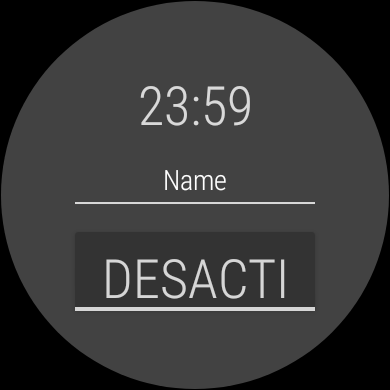
\includegraphics[width=\linewidth]{appActivity.png}
      \caption{Aplicación de gestión}
      \label{fig:uiActivity}
  \end{subfigure}
  \hfill
  \begin{subfigure}[b]{0.4\textwidth}
      \centering
      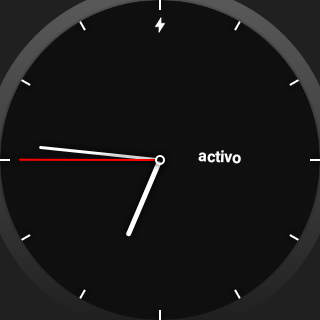
\includegraphics[width=\linewidth]{appWatchface.png}
      \caption{\textit{Watchface}}
      \label{fig:uiWatchface}
  \end{subfigure}
  \caption{\label{fig:ifell:UI} Interfaz de usuario de iFell}
\iffalse
\subfloat{\label{fig:uiActivity} Aplicación de gestión}{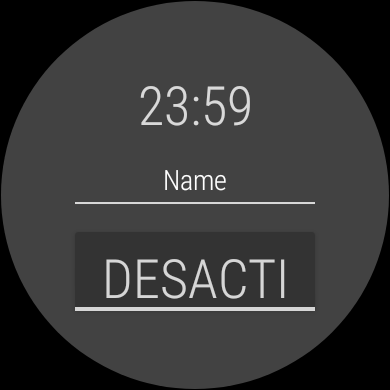
\includegraphics[width=0.4\linewidth]{appActivity.png}}
     \caption{\label{fig:uiApps} Interfaces de usuario}
     \hfill
\subfloat{\label{fig:uiWatchface} Watchface}{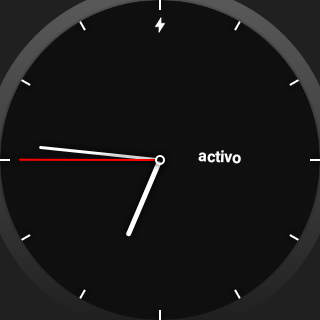
\includegraphics[width=0.4\linewidth]{appWatchface.png}}
\fi
\end{figure}


La aplicación toma forma de un objeto cotidiano e interactúa con el usuario utilizando un concepto conocido para este: un reloj digital. La única información que se muestra al usuario es la hora (adicionalmente el propio sistema operativo sobreimprime indicaciones de batería baja, ausencia de conexión a internet y existencia de notificaciones de otros servicios y aplicaciones). De esta forma, para el usuario, el dispositivo se convierte en un objeto conocido con un uso muy extendido que de forma adicional a su función tradicional realiza el proceso de detección de caídas.

En esta aplicación se han reducido al máximo las interacciones requeridas por parte del usuario en todo momento, hasta el punto de no requerir ninguna. La aplicación funciona en todo momento como un reloj tradicional mostrando la hora de forma analógica mediante unas manecillas. En el caso de detectarse una caída o evento similar, emitirá de forma automática una serie de avisos visuales, acústicos y hápticos (según las capacidades del dispositivo sobre el que se ejecute) que podrán ser desactivados si se detecta actividad nuevamente. Aunque también existe la posibilidad de desactivarlos tocando la pantalla.

La segunda interfaz que provee la aplicación se encarga de las tareas de administración y configuración. Permite introducir un nombre del usuario y forzar el estado de funcionamiento de los servicios de captura y detección. Si bien ninguno de estos procesos es necesario para el funcionamiento, se ofrece para facilitar la puesta en marcha y prueba del sistema.

\subsection{Comunicación con el Servidor}


% ########################################

El desafío de consolidar en un sistema portable una aplicación autónoma de detección de caídas debe hacer frente a una serie de limitaciones.

\section{Desafíos}
\todo{esto son requisitos, movel al punto anterior} El objetivo de todo modelo de detección de eventos es lograr un sistema que consiga capturar la totalidad de las realizaciones del mismo con el menos número posible de falsos positivos. En otras palabras, buscamos un sistema con una especificidad y sensibilidad de 100\%\cite{Noury2007}. \todo{Añadir referencias a papers, comentarios sobre sensibilidad y especificidad}.

\subsection{Usabilidad}\todo{de nuevo un requisito, al apartado anterior}
El primer reto de toda aplicación es conseguir una experiencia de usuario adaptada al cliente final. De nada sirve lograr implementar una plataforma que cumpla perfectamente con todos los requisitos y objetivos funcionales si el producto resultante se utiliza.

\subsubsection{Público objetivo}
Como se ha mencionado en la introducción del trabajo, los daños relacionados con las caídas son una de las principales causas de mortaldad entre las personas mayores de 65 años \todo{cita requerida}. Es propio de este grupo de población la desafección por la tecnología y la carencia o desinterés por su uso. Esta condición ha de ser tenida en cuenta para el desarrollo de cualquier producto.

Las personas de edad avanzada suelen padecer así mismo de otras condiciones que pueden limitar su grado de movilidad, atención o memoria que impidan o reduzcan la posibilidad de adaptarse o incorporar nuevas rutinas. Los problemas motores y de percepción reducen notablemente la capacidad de mostrar información así como de interactuar con el usuario cuando se necesite una acción por su parte.

Se entiende por tanto que si se ha de realizar un producto para esta población, es requisito que sea lo menos obtrusivo posible \todo{de nuevo un requisito, al punto anterior}, siendo recomendable incorporar la funcionalidad a un objeto de uso cotidiano para evitar la modificación de rutinas o la reticencia a incorporar nuevos procesos o elementos en su vida diaria. La interfaz de usuario debe ser mínima, usando un lenguaje visual que resulte familiar alejado de los estándares de las aplicaciones modernas. Así mismo, reducir o eliminar los procesos de configuración y manipulación, con un sistema que funcione al salir de la caja \todo{mala traducción de \textit{out of the box}}.

\subsubsection{Localización}

Una de las decisiones con mayor impacto sobre la funcionalidad del prototipo es la elección de la posición del dispositivo de captura ya que influencia en gran medida a la capacidad de detección de caídas \cite{Kangas2008}. Diversos estudios muestran que el mejor lugar para posicionar un sistema de medición de la aceleración para detectar caídas es la cintura, seguida de la cabeza siendo posible también usar un medidor en la muñeca\cite{Chen2005, Kangas2008, Noury2007}. Si bien estos resultados se basan en el análisis de métodos analíticos basados en cotas, se desprende de ellos la actitud o posición del cuerpo es un buen indicador para la predicción de actividades, razón por la que realizar la captura en muñecas o tobillos, las extremidades más alejadas del tronco, sufren de mayores penalizaciones para conseguir buenas estimaciones.

Al optarse por un reloj o \textit{pulsera de actividad} como plataforma para la implementación las opciones para posicionar la unidad de medida quedan reducida a una: la muñeca.

\subsection{Conectividad}

Hasta la fecha, los sistemas de detección de caídas se basan en arquitecturas cliente servidor para disociar el módulo de cómputo del de captura y conseguir que el dispositivo a llevar en si sea del menor tamaño posible. Este acercamiento que permite solventar el problema que derivaría de tener que llevar un obtrusivo sistema sobre si añade el problema de la necesidad de un enlace o comunicación con el módulo de cálculo. Ganamos en usabilidad pero perdemos en portabilidad.\todo{Cita y referencias a sistemas comerciales}

El principal problema de la conectividad radica en el hecho de que a pérdida de comunicación entre ambos módulos deriva en un sistema con ninguna capacidad. El módulo de cálculo, privado de datos no es capaz de realizar ninguna detección. Por su parte el aparato de captura, por si mismo, no tiene capacidad alguna para realizar nada más que la lectura.

El sistema implementado opta por una arquitectura cliente-pesado y servidor ligero. El cliente tiene suficiente capacidad para realizar captura, cómputo y capacidad de alerta como para funcionar de forma aislada. El servidor realiza funciones de expansión de la capacidad de alerta de la plataforma, así como de distribución de actualizaciones o mejoras en modelos y parámetros, pero de ninguna manera resulta imprescindible para el funcionamiento del dispositivo portable. Este es el principio básico y director de este trabajo: implementar una plataforma autónoma de detección de caídas capaz de ejecutarse en un dispositibo vestible.


\section{Plataforma}
\todo{justificar cada una de estas decisiones}
Para el servidor optamos por una arquitectura de microservicios usando la plataforma de AWS Lambda con almacenamiento en S3

Para el dispositivo móvil usamos un reloj inteligente Fossil Sport con sistema operativo WearOS y por tanto compatible con el ecosistema Android.

El la generación, entrenamiento, análisis y evaluación de modelos se realiza usando Keras/Tensorflow corriendo en la plataforma Google Colab.

\section{Arquitectura}\label{desc_archi}
\warn{según la profe punto muy interesante, a pulir }

\subsection{Arquitectura del sistema}

\warn{hablando de AWS: (ver siguiente páraffo)}
Resumiendo la estructura del sistema, \textit{AWS S3} (\url{https://aws.amazon.com/es/s3/?c=ser&sec=srv}) es el sistema de almacenamiento de datos en la red. Un disco duro en la nube, escalable en capacidad y fácilmente accesible para poder recuperar los datos. \textit{AWS Lambda} (\url{https://aws.amazon.com/es/lambda/?c=ser&sec=srv}) permite implementar funciones de código y definir una serie de eventos para lanzar su ejecución, al formar parte del ecosistema AWS es fácil conectar estas funciones con el sistema S3 y API Gateway. Finalmente \textit{AWS API Gateway} permite definir unos puntos de entrada, o URLs que conformarán la API del servicio. Cuando una de estas direcciones URL es invocada, inmediatamente se ejecuta la 



\todo{show me the data!!! cómo llegamos a 3G?}
El valor de $A_{umbral}$ se obtiene experimentalmente gracias al análisis de los datos obtenidos. Se fija en $A_{umbral} = 3G$ que resulta un buen equilibrio ya que conseguimos una cantidad reducida de eventos manteniendo un nivel bajo\todo{citar trabajos y medidas. Bourke usa 3,5G, otros usan valores más altos, la mayoría de caídas tienen niveles instantáneos de SVTot superiores a 6G}.\todo{incluir trabajo estadístico de los datos de aceleración del dataset} \todo{incluir gráfica temporal explicativa del algoritmo}

Si se sobrepasa el umbral en $t=0$. El sistema envía instantáneamente al siguiente modelo las muestras entre $t=-225$ y $t=-25$ (4 segudnos previos al evento). En segundo plano sigue capturando muestras hasta $t=25$. Este segundo bloque de 50 muestras (un segundo centrado en el evento) se envía también a la siguiente etapa. La decisión de separar el envío de datos a la siguiente etapa está motivada por la reducción de la latencia del sistema y obtener una clasificación o resultado con la menor dilación posible.


\subsubsection{Modelo RNN}


El modelo predictivo, se basa en la capacidad de las redes RNN y particularmente las basadas en celdas LSTM y GRU para generar modelos predictivos de calidad para series temporales de señales estacionarias \cite{Qin2019}.




\figura{trainingModeloRNN}{fig:rnnTrainAlt}{Evolución de RMSE durante el entrenamiento}

\figura{prediction.png}{fig:prediccionAceleracion}{Predicción de la aceleración}

\paragraph*{Detección}

Este segundo bloque recibe por un lado la señal $SVTot(-25:25)$\todo{no es un formato aceptable, usar t-25, t-24, .... t+25 o algo que sea aceptable} del acelerómetro y por el segundo la predicción $\hat{SVTot}(-25:25)$ \todo{unificat nomenclatura!!!}. Para clasificar el evento como una caída, usaremos un umbral sobre el error de predicción del modelo recurrente. La métrica de error empleada es la \textit{Raíz del Error Cuadrático Medio} definida como: \[
RECM=\sqrt{1/T\sum_{t_1}^{t_2}|y-\hat{y}|^2 }
\]Donde $t_1 = -25$, $t_2 = 25$ y $T=t_2-t_1=50$.

Comparando el resultado del error obtenido con un nuevo umbral al que denominaremos umbral de detección $U_{d}$ obtendremos finalmente la clasificación del evento en \textit{Caída} o \textit{no-Caida}. Dicho umbral se obtiene de nuevo de forma experimental.

En este caso el valor utilizado se calcula mediante el análisis del RECM usado durante la validación del modelo durante el entrenamiento. \todo{mostrar valores}

 
%Añade errores pero sobretodo son referencias

\chapter{Evaluación}\label{chap:eval}
% !TeX root = ../tfm.tex
%! TEX root = ../tfm.tex

Estudiaremos los resultados obtenidos por los desarrollos de este trabajo en dos bloques. En el primero analizaremos el algoritmo y modelos generados frente al estado del arte en modelos de detección de caídas y evaluaremos el grado de satisfacción de las metas deseadas. En segunda instancia introduciremos los resultados obtenidos con la aplicación \ifell/. Estudiaremos la viabilidad del acercamiento propuesto desde a nivel técnico y funcional así como la adecuación a solventar el problema y metas a lograr.

\section{Evaluación del modelo y algoritmo de \ifell/}

Un sistema de detección de caídas es en el fondo un clasificador con una única clase. Todos los resultados pueden por tanto agruparse en los que pertenecen o no a dicho conjunto. Con el fin de evaluar y comparar los resultados obtenidos usaremos dos métricas estadísticas:
\begin{itemize}
  \item Sensitividad (Capacidad de identificar las caídas), también conocida como \textit{recall}.
  \[
    Sensitividad = \frac{TP}{TP+FN}
  \]
  \item Especificidad o Selectividad (Capacidad de discernir únicamente las caídas).
  \[
    Especificidad = \frac{TN}{TN+FP}
  \]
\end{itemize}

Finalmente, como criterio de evaluación promediado de ambas en este trabajo hemos usado un promediado ponderado que daba mayor importancia a la sensibilidad sobre la especificidad pues tenemos como exigencia lograr un clasificador con la mayor sensibilidad posible. Sin embargo de cara a la evaluación usaremos la \textit{exactitud promediada} definida como:\[
  ExactitudPromediada=\frac{Sensibilidad+Especificidad}{2}
\]

Estas métricas son usadas habitualmente en otros trabajos similares\cite{Noury2007,Chen2005, Bourke2006} y permite utilizar los mismos indicadores para analizar los resultados de diferentes modelos directamente.

\subsection{Evaluación del algoritmo sobre SisFall}\label{sub:eval:hibrido}

\subsubsection{Metodología}

Partiendo del algoritmo de \ifell/ descrito en en \fullref{sec:imp:model}, usaremos un detector \textit{BourkeU} con cota de decisión fijada a 5g como modelo analítico y los modelos \textit{RNN-R(175)[50]}, \textit{RNN-P(175)[50]} y \textit{RNN-R(350)[50]} para el bloque de decisión final. Analizaremos los resultados para varios valores de la cota de decisión sobre el RMSE así como de la posición del punto de impacto $t_0$.

Recuperamos las mismas particiones de \sisfall/ hechas para el entrenamiento de los modelos que recordemos estaban conformadas con un 80\% para entrenamiento y el 20\% de muestras para validación. De la misma forma que analizamos el comportamiento del algoritmo de Bourke en la sección \ref{sub:imp:model:analitico} observaremos el comportamiento del algoritmo de modelo híbrido de \ifell/. Usando el subconjunto de entrenamiento para definir la cota de decisión sobre el error RMSE se la salida del modelo codificador/decodificador con la señal esperada y posteriormente evaluaremos los resultados obtenidos tras aplicar el algoritmo al conjunto de validación en relación a la literatura existente.

\subsubsection{Obtención de la cota del RMSE de decisión}

Alimentamos las tres variaciones elegidas con las sesiones del conjunto de validación y calculamos el RMSE para cada ejercicio de la base de datos. Almacenamos el resultado para poder calcular el histograma de manera similar a como hicimos con el modelo de Bourke.

\begin{figure}[!ht]
  \centering
  \begin{subfigure}[b]{0.31\textwidth}
      \centering
      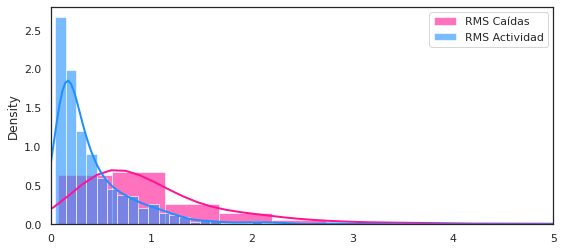
\includegraphics[width=\linewidth]{SISFALL175_RECON_RMS_HIST.png}
      \caption{\footnotesize \label{fig:ifell:sisfall:rmshist:175:recon}Distribuciones de RMSE para actividades y caídas en el modelo RNN-R(175)[50]}
  \end{subfigure}
  \hfill
  \begin{subfigure}[b]{0.31\textwidth}
      \centering
      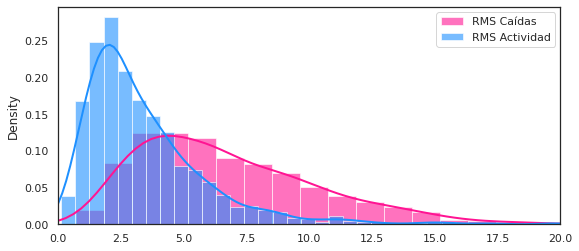
\includegraphics[width=\linewidth]{SISFALL175_PRED_RMS_HIST.png}
      \caption{\footnotesize \label{fig:ifell:sisfall:rmshisit:175:pred}Distribuciones de RMSE para actividades y caídas en el modelo RNN-P(175)[50]}
  \end{subfigure}
  \hfill
  \begin{subfigure}[b]{0.31\textwidth}
      \centering
      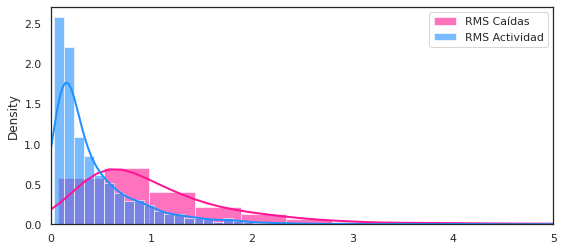
\includegraphics[width=\linewidth]{SISFALL350_RECON_RMS_HIST.png}
      \caption{\footnotesize \label{fig:ifell:sisfall:rmshist:350:pred}Distribuciones de RMSE para actividades y caídas en el modelo RNN-R(350)[50]}
  \end{subfigure}
  \caption{\footnotesize \label{fig:ifell:sisfall:rmshist}Histogramas del RMSE para actividades y caídas por modelo sobre \sisfall/}
\end{figure}



\tablas[0.7]{tab:eval:hibrid:percentiles}{Percentiles de caídas y actvidades para una misma cota de error RMSE}{lrrrrrrrr}{
                & \multicolumn{2}{c}{RNN-R(175)[50]}              & \multicolumn{2}{c}{RNN-P(175)[50]}         & \multicolumn{2}{c}{RNN-R(350)[50]} & \multicolumn{2}{c}{Bourke U} \\ \cmidrule(lr){2-3}\cmidrule(lr){4-5}\cmidrule(lr){6-7}\cmidrule(lr){8-9}
\textit{Caídas (\%)} & \textit{RMSE} &  \textit{Actividades (\%)} & \textit{RMSE} &  \textit{Actividades (\%)} & \textit{RMSE} &  \textit{Actividades (\%)} & $\|\vec{A}\|~(g)$ &  \textit{Actividades (\%)} \\\midrule
0                   &  0,0701        & 5,05                       & 0,6956        &  2,21                      & 0,0690        &  8,35                      &  4,1603           & 23,07 \\
1                   &  0,1404        & 27,21                      & 1,6145        &  19,71                     & 0,1432        &  30,05                     & 5,7755            & 41,32 \\
3                   &  0,2358        & 47,21                      & 1,9264        &  29,03                     & 0,2168        &  46,13                     & 6,6778            & 48,70 \\
5                   &  0,2822        & 52,78                      & 2,2176        &  36,87                     & 0,2676        &  53,35                     & 7,4037            & 54,38 \\
10                  &  0,3632        & 62,04                      & 2,7781        &  50,51                     & 0,3566        &  61,36                     & 9,6978            & 62,65 \\
}{2}

Comparando los resultados con los del modelo de Bourke, se observa un primer fenómeno de compresión del espacio de resultados: el rango de valores del RMSE es muy inferior al rango de valores pico usado para discriminar en Bourke. Si analizamos los datos de la tabla \ref{tab:eval:hibrid:percentiles}, se observa como el comportamiento de los dos modelos de reconstrucción es muy similar a pesar de la diferencia en el tamaño de las redes. Al mismo tiempo, se observa una mayor capacidad de discriminación de caídas y actividades que con respecto al modelo de predicción de hasta 17 puntos.  Haciendo del modelo RNN-R(175)[50] un muy buen candidato para el sistema por equilibrar capacidad de clasificación con consumo de recursos. Calculamos la Exactitud Promediada de cada variación para obtener el mejor clasificador tal y recopilamos los resultados en la tabla \ref{tab:eval:sisfall:best}. El modelo RNN-R(175)[50] se muestra como el mejor clasificador en relación a la exactitud promediada.

\tablas{tab:eval:sisfall:best}{Sensibilidad, Especificidad y Exactitud Promediada para el mejor caso de cada modelo}{lrrrrr}{
  \textit{Modelo} & \textit{ExactitudP.} & \textit{Sensibilidad} & \textit{Especificidad} & $\Delta t$ & \textit{RMSE} \\ \midrule
  RNN-R(175)[50]  & 81,4                & 97,2                   & 65,6                   & -50        & 0,2822 \\
  RNN-P(175)[50]  & 76,5                & 91,6                   & 61,5                   &   0         & 2,2176 \\
iRNN-R(350)[50]    & 79,5                & 96,1                   & 63,0                   & -50        & 0,2676 \\
}{2}


\subsection{Evaluación del algoritmo}




En los requisitos a cumplir por nuestro clasificador hemos indicado que debe ofrecer unos resultados equiparables a los del estado del arte 



%%%% Esto lo pondremos en el apartado evaluación.
Observamos la mejora del modelo de predicción, que manteniendo la sensibilidad logra superar por hasta un 8\% la especificidad del clasificador equivalente. Si observamos las matrices de confusión de las figura \ref{fig:ifell:adata:confmats}  se aprecia como ya hemos mencionado que la sensibilidad del algoritmo no alcanza nunca el 100\% pero que esta penalización debida al modelo de Bourke previo no impacta en cuanto decidimos reducir la sensibilidad del algoritmo para mejorar la especificidad.


\begin{sidewaysfigure}[!ht]
  \centering
  \begin{subfigure}[b]{0.45\textwidth}
      \centering
      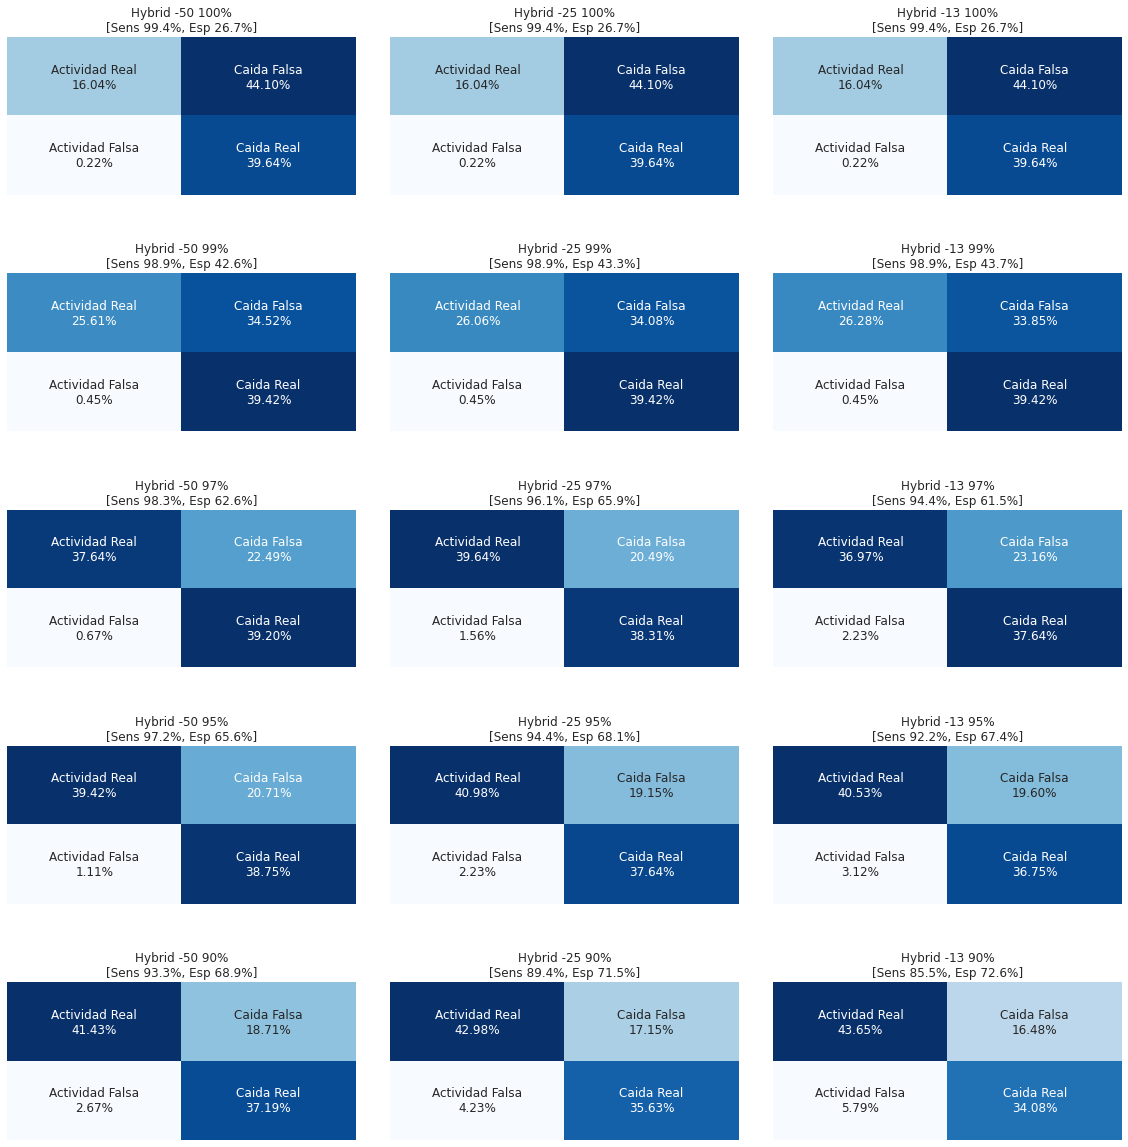
\includegraphics[width=\linewidth]{ConfMatrixRecon.png}
      \caption{\footnotesize \label{fig:ifell:adata:confmat:recon}Matrices de confusión para un modelo de reconstrucción}
  \end{subfigure}
  \hfill
  \begin{subfigure}[b]{0.45\textwidth}
      \centering
      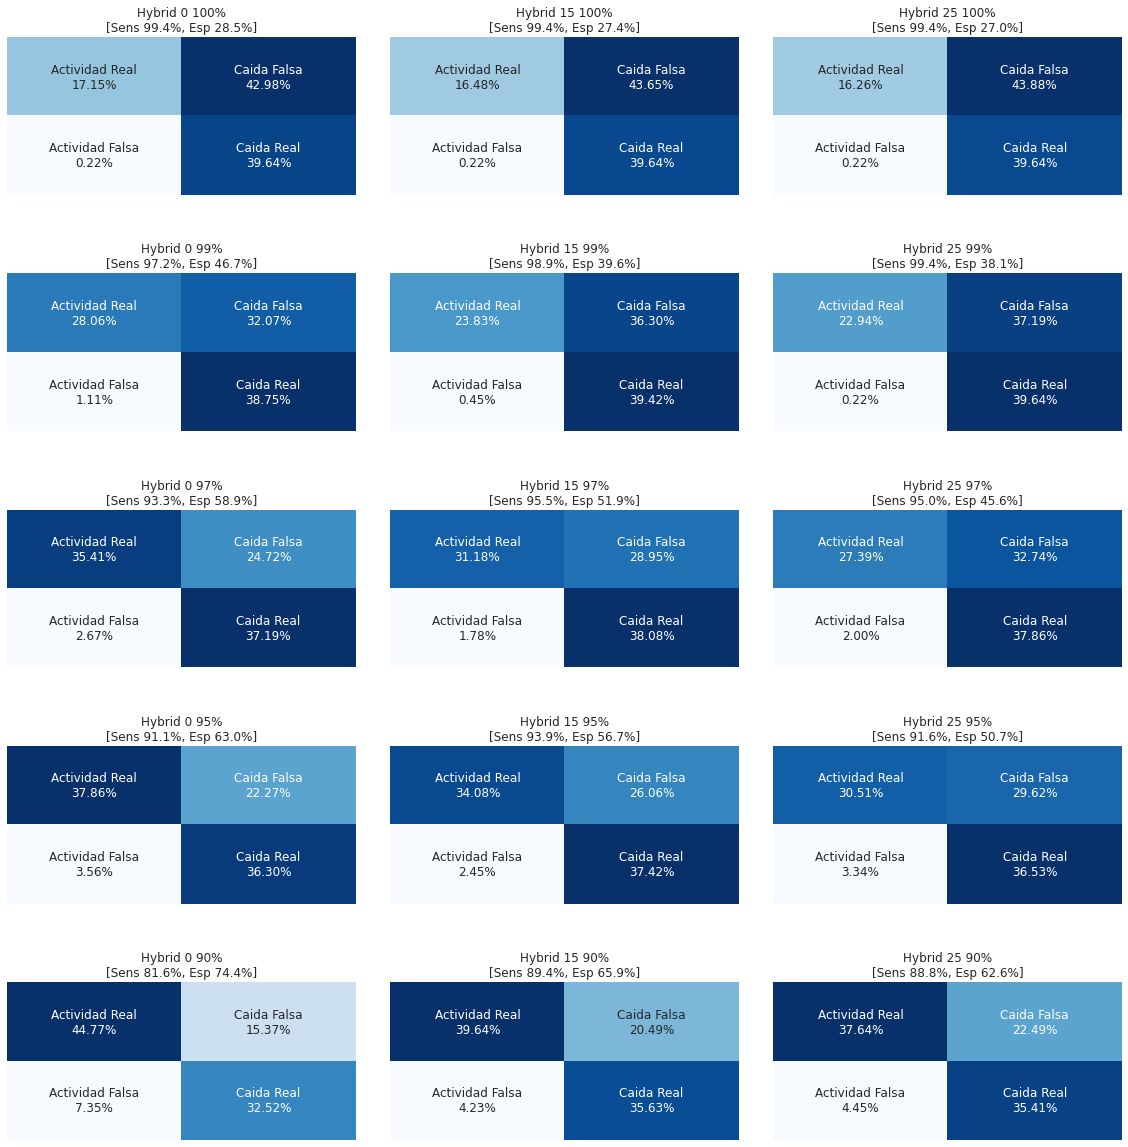
\includegraphics[width=\linewidth]{ConfMatrixPred.png}
      \caption{\footnotesize \label{fig:ifell:adata:confmat:pred}Matrices de confusión para un modelo de predicción}
  \end{subfigure}
  \caption{\label{fig:ifell:adata:confmats}Ejemplos de matrices de confusión según sensibilidad deseada y posición de la ventana}
\end{sidewaysfigure}


\begin{figure}[!ht]
  \centering
  \begin{subfigure}[b]{0.45\textwidth}
      \centering
      \includegraphics[width=\linewidth]{ADATA_RECON_RMSE_HIST}
      \caption{\footnotesize \label{fig:ifell:adata:rmshist:recon}Distribuciones de RMSE para actividades y caídas en el modelo de reconstrucción}
  \end{subfigure}
  \hfill
  \begin{subfigure}[b]{0.45\textwidth}
      \centering
      \includegraphics[width=\linewidth]{ADATA_PRED_RMS_HIST}
      \caption{\footnotesize \label{fig:ifell:adata:rmshist:pred}Distribuciones de RMSE para actividades y caídas en el modelo predicción}
  \end{subfigure}
  \caption{\label{fig:ifell:adata:rmshist}Histogramas del RMSE para los modelos IFELL}
\end{figure}

En la tabla \ref{tab:MLResults} Destacan los buenos resultados obtenidos por los modelos que usan técnicas de aprendizaje automático. Si bien en lo referente a la latencia, \cite{Liu2020} obtiene tiempos que superan el segundo en la mayoría de modelos, llegando incluso a los 8,87s obtenidos con un clasificador de Bayes. Tanto en los trabajos de \cite{Liu2018, Liu2020} como \cite{Musci2020} y \cite{Torti2018} se subraya el hecho de la no uniformidad de los resultados. Los mejores resultados se obtienen con población joven mientras que con población adulta las métricas pueden perder hasta 5 puntos, en parte debido a la falta de datos de entrenamiento. En la tabla \ref{tab:eval:resultados} se muestran los resultados de este estudio junto con los arriba mencionados y los propios resultados del estudio de \sisfall/\cite{Sucerquia2017}. Existe también el trabajo de \citeA{Putra2017} pero en su publicación no ofrece datos suficientes para obtener las métricas de especificidad, aunque clama una sensibilidad del 99,9\%. Salvo los estudios de Musci y Torti, el resto de los modelos se ejecutan en grandes equipos. Es obvio que el clasificador obtenido no alcanza la exactitud de los mejores modelos de aprendizaje automático, aunque se muestra superior a Bayes. Muestra sin embargo mejores estadísticas que los modelos analíticos sin información de la posición como Bourke y muy similar a modelos estadísticos que analizan largas secuencias. Destacamos asímismo los rápidos tiempos de ejecución de los modelos (ejecutados en los sistemas descritos en el apéndice \ref{app:colab}), un orden de magnitu mejor que el modelo CNN y dos órdenes mejor que el modelo LSTM presentados Liu. Dadas las limitaciones por los requisitos de recursos y latencia del sistema consideramos los resultados obtenidos por los clasificadores de \ifell/ satisfactorios.

% \tablas[0.80]{tab:MLResults}{Resultados de sistemas basados en ML}{lccccccccc}{
%     & \multicolumn{2}{c}{\textbf{iFell}}  & Musci2020     & Torti2018  & \multicolumn{3}{c}{Liu} &  \multicolumn{2}{\sisfall} & Bourke \\ \cmidrule{lr}{2-3}\cmidrule{lr}{4}\cmidrule{lr}{5-7}\cmidrule{lr}{8-9}
%     & Rec.  & Pred.           & LSTM & LSTM   & FD-DNN    & LSTM     & CNN   & SVM. & Best  & SVM \\ \midrule
% Sensitividad (\%) & 97,2  & 94,4          &   96,53   & 98,73       & 94,09     & 81,47   & 87,50 & \~99,99 &\~99,99  & 99,4 \\
% Especificidad (\%)& 65,6  & 63,0          &    96,01  & 97,93       & 99,94     & 99,57   & 99,88 & 32,97 & 67,97     & 29,7 \\
% Exactitud (\%)    &       &               &           & 98,33       & 99,17     & 96,88   & 98,13 & 66,43 & 83,96     & \\
% Exactitud Prom(\%)& 81,4  &               &    96,27  & 98,33       & 96,63     & 90,52   & 98,13 &       &           & 64,55\\
% Tiempo(s)         & 0,065 & 0,060         &           &             & 1,05      & 3,87    & 0,65  &  0    &           & 0\\
% }{3}

\tablan{tab:eval:resultados}{Métricas de detectores de caídas usando \sisfall/}{llccccc}{
  \emph{Estudio} & \emph{Modelo} & \emph{Sens}. & \emph{Especif.} & \emph{Exactitud} & \emph{Exact. Pond.} & \emph{Tiempo (s)} \\ \midrule
  \multirow{5}{*}{\ifell/} & RNN-R(175)[50] & 97,2  & 65,6  &     & 81,4 & 0,035 \\ 
                           & RNN-P(175)[50] & 94,4  & 63,0  &     & 78,7 & 0,031 \\
                           & IFELL-R(175)[50] & 97,8 & 65,6 &     & 82,2 & 0,035 \\
                           & IFELL-P(175)[50] & 90,5 & 68,9 &     & 79,7 & 0,031 \\
                           & Bourke & 99,4 & 29,7 &  & 64,5 & 0,0\\ \midrule[0.1]
    Musci2020                 & LSTM            & 96,5  & 96,0  &     & 92,7 & \\ \midrule[0.1]
    Torti2018                 & LSTM            & 98,7  & 97,9  & 98,3& 98,3 & \\\midrule[0.1]

    \multirow{5}{*}{Liu2018}  & SVML\tnote{1} & 97,2   & 93,6  & 95,4& 95,4 & \\
                              & SVMRBF\tnote{2} & 98,3 & 96,2 & 97,6 & 97,2 & \\
                              & kNN3   & 96,4 & 96,3 & 96,4 & 96,3 & \\
                              & Bayes  & 54,3 & 92,0 & 73,7 & 73,1 & \\
                              & DT\tnote{3} & 94,9 & 95,5 & 95,2 & 95,2 & \\\midrule[0.1]

    \multirow{3}{*}{Liu2020} & FD-DNN\tnote{4} & 94,1 & 99,9 & 99,1 & 97,0 & 1,05 \\
                             & LSTM & 81,4 & 99,5 & 96,88 & 90,4 & 3,87 \\
                             & CNN & 87,5 & 99,9 & 98,1 & 93,7 & 0,65 \\
                             & Bayes & 95,6 & 99,9 & 90,1 & 97,7 & 8,87 \\
                             & RT\tnote{5} & 92,2 & 98,5 & 80,32 & 95,3  & 1,21 \\ \midrule[0.1]

    \multirow{2}{*}{\sisfall/} & NormAcc\tnote{6} & \~99,9 & 32,97 & 66,4 & 66,4 & \\
                               & STDEV\tnote{7} & \~99,9 & 67,97 & 83,96 & 83,96 & \\
}{
\item [1] SVM Linear 
\item [2] SVM Radial Basis Function
\item [3] Decission Trees
\item [4] Deep Neural Network for Fall Detection
\item [5] Random Trees
\item [6] Norma de la aceleración en plano horizontal
\item [7] Desviación estándar del módulo
}{21}

\figura{CompositeFallNormalRMSHistogram_t-25}{fig:GRU_predictionRMS_Histogram}{Histograma de los errores de predicción del modelo GRU}

\paragraph{\ifell/ respecto a Bourke}\\
El comparador de Bourke es usado por nuestro algoritmo a modo de generador de eventos. Es además un referente en los modelos analíticos que usan el módulo de la aceleración por lo que es adecuado analizar el algoritmo de \ifell/ contra el modelo de Bourke ya que nos indicará el grado de mejora debido al desarrollo realizado. Tomaremos la variante que analiza únicamente los picos de la aceleración pues el que ha mostrado mejor comportamiento. Si forzamos una alta sensibilidad tal que $Sensibilidad \geq 99\%$ los resultados muestran una clara mejoría en la capacidad selectiva del algoritmo híbrido de \ifell/ de reconstrucción respecto al modelo de Bourke del 41\%. 

  \tablas{tab:ifell:vs:bourke}{Especificidad por modelos forzando $Sensibilidad \geq 99\%$}{lrr}{
    \emph{Modelo}     & \emph{Sensibilidad} & \emph{Especificidad} \\ \midrule
    Bourke U          & 99,0\%    & 41,3 \% \\                
    IFELL-R(175)[50]    & 99,0\%  & 58,5 \% \\
    IFELL-P(175)[50]    & 99,0\%  & 48,9 \% \\
  }{2}

\section{Evaluación de la aplicación \ifell/}

  Finalmente debemos evaluar la implementación del sistema. Partiendo del algoritmo de \ifell/ descrito en en \fullref{sec:imp:model}, e implementado en la aplicación \ifell/ usaremos un detector \textit{BourkeU} con cota de decisión en 5g como modelo analítico y los modelos \textit{IFELL-R(175)[50]} e \textit{IFELL-P(175)[50]} con cotas de decisión sobre RMSE fijadas a $RMSE_{Pred}=2,2176$ y $RMSE_{Recon}=0,2822$, es decir, buscando conseguir el 95\% de sensibilidad.

\subsection{Latencia}
    La aplicación con la configuración descrita se ha probado en un sujeto durante un periodo de dos meses de uso continuo sin pausas más allá de los periodos de carga del dispositivo. En todo este periodo no se ha producido ninguna caída real y 12 falsos positivos, la ausencia de casos positivos reales no permite realizar un análisis estadístico. Si que podemos estudiar las latencias o tiempos de ejecución del modelo recogidos en la tabla \ref{tab:ifell:watch:latencia}. Para ello medimos el tiempo desde que se invoca la petición al modelo hasta que obtenemos el resultado del comparador del nivel de decisión RMSE. 

    \tablas{tab:ifell:watch:latencia}{Tiempo de cómputo de \ifell/ en el dispositivo Fossil Sport Gen.3}{lrr}{
        \textit{Modelo}  & \textit{Float16} & \textit{Dinámico} \\ \midrule
        IFELL-P(175)[50] & 2,785 s   & 1,206 s \\
        IFELL-R(175)[50] & 2,538 s   & 1,303 s \\
        IFELL-R(350)[50] & 5,185 s   & 2,826 s \\
      }{2}

      Se aprecia el interés en optimizar los modelos para su ejecución en dispositivos embebidos. Al ser un dispositivo con una unidad GPU de capacidad limitada es la optimización a enteros don rango dinámico la que ofrece mejor tiempo de respuesta. Es notable haber conseguido unos tiempos de respuesta cercanos al segundo en un dispositivo llevable cuando tal y como se recoge en la tabla \ref{tab:eval:resultados} algunos de los modelos comparados necesitan siete veces más tiempo en un potente sistema de sobremesa. 

\subsection{Adecuación de la solución}
El objetivo de todo modelo de detección de eventos es lograr un sistema que consiga capturar la totalidad de las realizaciones del mismo con el menos número posible de falsos positivos. En otras palabras, buscamos un sistema con una especificidad y sensibilidad de 100\%\cite{Noury2007}. En el caso del sistema \ifell/ hemos optado por un enfoque que prime la facilidad de uso y sensibilidad por encima de otros aspectos. Es decir, dada una experiencia de usuario desarrollamos una aplicación que maximizase la capacidad de detección de caídas.

\subsubsection{Público objetivo}
Para definir la experiencia de usuario primero analizamos quién era el usuario objetivo. Como se ha mencionado en la introducción del trabajo, los daños relacionados con las caídas son una de las principales causas de mortaldad entre las personas mayores de 65 años. Es propio de este grupo de población la desafección por la tecnología y la carencia o desinterés por su uso. Esta condición ha de ser tenida en cuenta para el desarrollo de cualquier producto.

Las personas de edad avanzada suelen padecer así mismo de otras condiciones que pueden limitar su grado de movilidad, atención o memoria que impidan o reduzcan la posibilidad de adaptarse o incorporar nuevas rutinas. Los problemas motores y de percepción reducen notablemente la capacidad de mostrar información así como de interactuar con el usuario cuando se necesite una acción por su parte.

Se entiende por tanto que si se ha de realizar un producto para esta población, es requisito que sea lo menos obtrusivo posible, siendo recomendable incorporar la funcionalidad a un objeto de uso cotidiano para evitar la modificación de rutinas o la reticencia a incorporar nuevos procesos o elementos en su vida diaria. La interfaz de usuario debe ser mínima, usando un lenguaje visual que resulte familiar alejado de los estándares de las aplicaciones modernas. Así mismo, reducir o eliminar los procesos de configuración y manipulación, con un sistema que funcione desde la primera ejecución.

\subsubsection{Plataforma y localización}
Teniendo en cuenta los requisitos anteriores optamos por un objeto vestible de uso cotidiano. Un complemento al que el usuario esté acostumbrado que sería reemplazado por el sistema desarrollado. Optamos por desarrollar el sistema sobre un reloj inteligente. Este objeto se asemeja en forma y función a los tradicionales relojes mecánicos y automáticos a los que la población adulta les resulta familiar y conocido. La recarga de la batería, único punto diferencial con respecto a los relojes tradicionales, no dista mucho de la necesidad de remontar el mecanismo de reserva de energía mecánica de sus homólogos no computerizados.

Esta decisión es la que tendrá mayor impacto sobre la funcionalidad del prototipo ya que fuerza la posición del dispositivo de captura. Diversos estudios muestran que el mejor lugar para posicionar un sistema de medición de la aceleración para detectar caídas es la cintura, seguida de la cabeza siendo desaconsejado usar sensores en las extremidades por su alta movilidad\cite{Chen2005, Kangas2008, Noury2007}. Al usar un reloj, y por tanto posicionar los sensores en la muñeca no sólo estamos penalizando la calidad de las lecturas sino que reducimos la capacidad de obtener información de la actitud o postura del cuerpo. Esta información permite desarrollar índices de detección analíticos de muy alta calidad, sin embargo por la posición tendremos que usar métodos basados únicamente en la norma del vector aceleración.

A juicio del autor, la penalización cualitativa resultante de dicha decisión queda compensada por la usabilidad de la plataforma. El mejor de los detectores de caídas resulta inútil si el usuario no lo utiliza. A este respecto, ninguno de los sujetos del ensayo tuvo problema alguno para manipular el sistema, a pesar de ser una muestra demasiado reducida para ser significativa.

\subsubsection{Interfaz y autonomía}
\figura{appBatt}{fig:ifell:bateria}{Consumo de batería}
La necesidad de interacción del usuario con el sistema es mínima y siempre opcional. Instalar la aplicación significa configurar una determinado aspecto de la esfera del reloj que presenta un aspecto analógico tradicional con manecillas para indicar horas, minutos y segundos y un pequeño mensaje de estado. Esta opción garantiza que el propio sistema operativo lanzará la aplicación tras cada arranque. A su vez los servicios necesarios se ejecutan siempre en segundo plano de manera que incluso si se usa otra aplicación en el dispositivo la detección de caídas sigue en marcha. Las única manipulación necesaria con el objeto es el proceso de carga. Con el fin de maximizar el tiempo entre cargas y con la meta de conseguir al menos 24 horas de autonomía se optó por un enfoque de modelo híbrido. En la \autoref{fig:ifell:bateria} se mostramos una captura de la pantalla de gestión de la batería del sistema operativo del reloj tras un día de uso con \ifell/ ejecutándose. Es un caso extremo ya que durante ese periodo no no se usó el reloj ni se encendió la pantalla en ningún momento. Sin embargo muestra que es fácil mantener 24 horas de actividad entre cargas sin problema. Este resultado es una clara mejoría con respecto a los experimentos previos como \citeA{Liu2020} en que el módulo de captura únicamente tiene una duración de 30 horas en envío de datos a la unidad de proceso, o las 20 horas de la unidad llevable que auna cómputo y medición propuesta por \citeA{Torti2018}. Confirmamos que la elección del algoritmo híbrido de detección ha resultado instrumental en conseguir modelos de muy alta eficiencia energética.




\chapter{Conclusiones y Trabajo Futuro}\label{chap:conclusiones}
% !TeX root = ../tfm.tex
%! TEX root = ../tfm.tex
\documentclass[../tfm.tex]{subfiles}
\begin{document}

\section{Conclusiones}

\section{Lineas de trabajo futuro}

Lineas de trabajo que podrían aportar valor al TFM realizado. Perspectivas de futuro que abre el trabajo realizado. Justificar en qué modo puede emplearse la aportación desarrollada y en qué campos.

\end{document}




% \bibliographystyle{unsrt}
% \bibliographystyle{apalike}
\newpage %necesario? parece que con apacite si
\bibliographystyle{apacite} % usa apacite y parece no funcionar, pero es el bueno
\bibliography{tfm}

\lstlistoflistings

\appendix

\chapter{Captura de datos y construcción del dataset}\label{app:dataset}
% \subfile{seccion/app-accelcapture}

\chapter{Listados de código}\label{app:codigo}
% !TeX root = ../tfm.tex
%! TEX root = ../tfm.tex
\section{AccelCapture}
\subsection{Servidor/Api Lambda}\label{app:code:accelcapturelambda} 
\subsubsection{POST guardarSesions}
% \begin{spacing}{0.5}
\todo{poner el nombre que toca a la función}
\lstinputlisting[style=ES6,caption={Listado de código de POST guardarSessions}]{code/lambdaAccelCapture.js}
% \end{spacing}

\section{iFell}
\subsection{Modelo RNN}
\subsubsection{Prunable Bidir}\label{app:code:ifell:prunebidir}
\lstinputlisting[language=Python,caption={Listado de código de implementación de capas PruneBidir]{code/pruneBidir.py}



\chapter{Plataforma Hardware}\label{app:plataforma}
\subfile{seccion/app-fossil}

\chapter{Artículo}
\includepdf[pages=-]{articulo.pdf} %descomentar cuando esté el artículo terminado.

% ELIMINAR EN VERSIÓN FINAL
% \listoftodos
\end{document}
